\documentclass[leqno, openany]{memoir}
\setulmarginsandblock{3.5cm}{3.5cm}{*}
\setlrmarginsandblock{3cm}{3.5cm}{*}
\checkandfixthelayout

\usepackage{amsmath}
\usepackage{amssymb}
\usepackage{amsthm}
%\usepackage{MnSymbol}
\usepackage{bm}
\usepackage{accents}
\usepackage{mathtools}
\usepackage{tikz}
\usetikzlibrary{calc}
\usetikzlibrary{automata,positioning}
\usepackage{tikz-cd}
\usepackage{forest}
\usepackage{braket} 
\usepackage{listings}
\usepackage{mdframed}
\usepackage{verbatim}
\usepackage{physics}
\usepackage{stmaryrd}
\usepackage{mathrsfs} 
\usepackage[normalem]{ulem} 
\usepackage{stackengine}
%\usepackage{/home/patrickl/homework/macaulay2}

%font
\usepackage[sc]{mathpazo}
\usepackage{eulervm}
\usepackage[scaled=0.86]{berasans}
\usepackage{inconsolata}
\usepackage{microtype}

%CS packages
\usepackage{algorithmicx}
\usepackage{algpseudocode}
\usepackage{algorithm}

% typeset and bib
\usepackage[english]{babel} 
\usepackage[utf8]{inputenc} 
\usepackage[T1]{fontenc}
\usepackage[bookmarks, colorlinks, breaklinks]{hyperref} 
\hypersetup{linkcolor=blue,citecolor=magenta,filecolor=black,urlcolor=blue}
\usepackage{cleveref}
\usepackage[backend=biber,style=alphabetic,maxalphanames=4,maxnames=5,hyperref,backref=true,backrefstyle=none]{biblatex}
\usepackage{xpatch}
\xpatchbibmacro{pageref}{parens}{backrefparens}{}{}
\crefname{equation}{}{}

% other formatting packages
\usepackage{float}
\usepackage{booktabs}
\usepackage[shortlabels]{enumitem}
\usepackage{csquotes}
\usepackage{titlesec}
\usepackage{titling}
\usepackage{parskip}
\usepackage{graphicx}
\graphicspath{{./}}

\usepackage{lipsum}

% delimiters
\DeclarePairedDelimiter{\gen}{\langle}{\rangle}
\DeclarePairedDelimiter{\floor}{\lfloor}{\rfloor}
\DeclarePairedDelimiter{\ceil}{\lceil}{\rceil}


\newtheorem{thm}{Theorem}[section]
\newtheorem{cor}[thm]{Corollary}
\newtheorem{prop}[thm]{Proposition}
\newtheorem{lem}[thm]{Lemma}
\newtheorem{conj}[thm]{Conjecture}
\newtheorem{quest}[thm]{Question}
\newtheorem{prob}[thm]{Problem}

\theoremstyle{definition}
\newtheorem{defn}[thm]{Definition}
\newtheorem{defns}[thm]{Definitions}
\newtheorem{con}[thm]{Construction}
\newtheorem{exm}[thm]{Example}
\newtheorem{exms}[thm]{Examples}
\newtheorem{notn}[thm]{Notation}
\newtheorem{notns}[thm]{Notations}
\newtheorem{addm}[thm]{Addendum}
\newtheorem{exer}[thm]{Exercise}

\theoremstyle{remark}
\newtheorem{rmk}[thm]{Remark}
\newtheorem{rmks}[thm]{Remarks}
\newtheorem{warn}[thm]{Warning}
\newtheorem{sch}[thm]{Scholium}


% unnumbered theorems
\theoremstyle{plain}
\newtheorem*{thm*}{Theorem}
\newtheorem*{prop*}{Proposition}
\newtheorem*{lem*}{Lemma}
\newtheorem*{cor*}{Corollary}
\newtheorem*{conj*}{Conjecture}

% unnumbered definitions
\theoremstyle{definition}
\newtheorem*{defn*}{Definition}
\newtheorem*{exer*}{Exercise}
\newtheorem*{defns*}{Definitions}
\newtheorem*{con*}{Construction}
\newtheorem*{exm*}{Example}
\newtheorem*{exms*}{Examples}
\newtheorem*{notn*}{Notation}
\newtheorem*{notns*}{Notations}
\newtheorem*{addm*}{Addendum}


\theoremstyle{remark}
\newtheorem*{rmk*}{Remark}

% shortcuts
\newcommand{\Ima}{\mathrm{Im}}
\newcommand{\A}{\mathbb{A}}
\newcommand{\F}{\mathbb{F}}
\newcommand{\E}{\mathbb{E}}
\newcommand{\G}{\mathbb{G}}
\newcommand{\N}{\mathbb{N}}
\newcommand{\R}{\mathbb{R}}
\newcommand{\C}{\mathbb{C}}
\newcommand{\Z}{\mathbb{Z}}
\newcommand{\Q}{\mathbb{Q}}
\renewcommand{\k}{\Bbbk}
\renewcommand{\L}{\mathbb{L}}
\renewcommand{\P}{\mathbb{P}}
\newcommand{\M}{\overline{M}}
\newcommand{\g}{\mathfrak{g}}
\newcommand{\h}{\mathfrak{h}}
\newcommand{\n}{\mathfrak{n}}
\renewcommand{\b}{\mathfrak{b}}
\newcommand{\ep}{\varepsilon}
\newcommand*{\dt}[1]{%
   \accentset{\mbox{\Huge\bfseries .}}{#1}}
\renewcommand{\abstractname}{Official Description}
\newcommand{\mc}[1]{\mathcal{#1}}
\newcommand{\T}{\mathbb{T}}
\newcommand{\mf}[1]{\mathfrak{#1}}
\newcommand{\mr}[1]{\mathrm{#1}}
\newcommand{\ms}[1]{\mathsf{#1}}
\newcommand{\mt}[1]{\mathtt{#1}}
\newcommand{\on}[1]{\operatorname{#1}}
\newcommand{\ol}[1]{\overline{#1}}
\newcommand{\ul}[1]{\underline{#1}}
\newcommand{\wt}[1]{\widetilde{#1}}
\newcommand{\wh}[1]{\widehat{#1}}
\renewcommand{\div}{\operatorname{div}}
\newcommand{\bir}{\sim_{\mr{bir}}}
\newcommand{\stacks}[1]{\href{https://stacks.math.columbia.edu/tag/#1}{#1}}
\newcommand{\ostar}{\stackMath\mathbin{\stackinset{c}{0ex}{c}{0ex}{\star}{\bigcirc}}}

\DeclareMathOperator{\Der}{Der}
\DeclareMathOperator{\Def}{Def}
\DeclareMathOperator{\Bl}{Bl}
\DeclareMathOperator{\NE}{NE}
\DeclareMathOperator{\Tor}{Tor}
\DeclareMathOperator{\Hom}{Hom}
\DeclareMathOperator{\Ext}{Ext}
\DeclareMathOperator{\End}{End}
\DeclareMathOperator{\ad}{ad}
\DeclareMathOperator{\Aut}{Aut}
\DeclareMathOperator{\Rad}{Rad}
\DeclareMathOperator{\Pic}{Pic}
\DeclareMathOperator{\supp}{supp}
\DeclareMathOperator{\Supp}{Supp}
\DeclareMathOperator{\sgn}{sgn}
\DeclareMathOperator{\spec}{Spec}
\DeclareMathOperator{\Spec}{Spec}
\DeclareMathOperator{\proj}{Proj}
\DeclareMathOperator{\Proj}{Proj}
\DeclareMathOperator{\ord}{ord}
\DeclareMathOperator{\Div}{Div}
\DeclareMathOperator{\depth}{depth}
\DeclareMathOperator{\coker}{coker}
\DeclareMathOperator{\ch}{ch}
\DeclareMathOperator{\Hilb}{Hilb}

% Section formatting
\titleformat{\section}
    {\Large\sffamily\scshape\bfseries}{\thesection}{1em}{}
\titleformat{\subsection}[runin]
    {\large\sffamily\bfseries}{\thesubsection}{1em}{}
\titleformat{\subsubsection}[runin]{\normalfont\itshape}{\thesubsubsection}{1em}{}

\title{COURSE TITLE}
\author{Lectures by INSTRUCTOR, Notes by NOTETAKER}
\date{SEMESTER}

\newcommand*{\titleSW}
    {\begingroup% Story of Writing
    \raggedleft
    \vspace*{\baselineskip}
    {\Huge\itshape Integrability, Enumerative Geometry, and Quantization \\ August-September 2022}\\[\baselineskip]
    {\large\itshape Notes by Patrick Lei}\\[0.2\textheight]
    {\Large Lectures by Various}\par
    \vfill
    {\Large \sffamily Simons Center for Geometry and Physics}
    \vspace*{\baselineskip}
\endgroup}
\pagestyle{simple}

\chapterstyle{ell}


%\renewcommand{\cftchapterpagefont}{}
\renewcommand\cftchapterfont{\sffamily}
\renewcommand\cftsectionfont{\scshape}
\renewcommand*{\cftchapterleader}{}
\renewcommand*{\cftsectionleader}{}
\renewcommand*{\cftsubsectionleader}{}
\renewcommand*{\cftchapterformatpnum}[1]{~\textbullet~#1}
\renewcommand*{\cftsectionformatpnum}[1]{~\textbullet~#1}
\renewcommand*{\cftsubsectionformatpnum}[1]{~\textbullet~#1}
\renewcommand{\cftchapterafterpnum}{\cftparfillskip}
\renewcommand{\cftsectionafterpnum}{\cftparfillskip}
\renewcommand{\cftsubsectionafterpnum}{\cftparfillskip}
\setrmarg{3.55em plus 1fil}
\setsecnumdepth{subsection}
\maxsecnumdepth{subsection}
\settocdepth{subsection}

\addbibresource{../../math.bib}
\DefineBibliographyStrings{english}{
    backrefpage={$\leftarrow$},
    backrefpages={$\leftarrow$},
}

\begin{document}
    
\begin{titlingpage}
\titleSW
\end{titlingpage}

\thispagestyle{empty}
\section*{Disclaimer}%
\label{sec:disclaimer}

These notes were taken during the program using the \texttt{vimtex} package of the editor \texttt{neovim}. 
Any errors are mine and not the speakers'. 
In addition, my notes are picture-free (but will include commutative diagrams) and are a mix of my mathematical style and that of the lecturers. Also, notation may differe between lecturers.
If you find any errors, please contact me at \texttt{plei@math.columbia.edu}.

\section*{Acknowledgements}

I would like to thank Ga\"etan Borot, Alexandr Buryak, Melissa Liu, Nikita Nekrasov, Paul Norbury, and Paolo Rossi for organizing this program.

\vspace*{1cm}

\noindent\textbf{Program Website:}  \url{https://scgp.stonybrook.edu/archives/33309}
\newpage

\tableofcontents

\chapter{Virasoro constraints in enumerative geometry (Alexei Oblomkov)}%
\label{cha:alexei}

Here is an equation of a plane curve over formal power series in $s$, which we will call the \textit{Lambert curve}:
\[ ye^y = xe^x e^{-s}. \]
This curve appears in the work of Oblomkov-Okounkov-Pandharipande~\cite{gwptdescendent} which treats the descendent Gromov-Witten/Pandharipande-Thomas correspondence in the stationary, non-fully equivariant case. The main question is to consider deformations of this curve.

We will now state the main formula of interest:
\begin{equation}\label{eqn:maineqn} 
    H^{\mr{GW}}(x) = \frac{x}{\theta} \Res_{w=\infty} \qty(\frac{\sqrt{\dd{y} \dd{w}}}{y-w}; e^{\theta \phi(y) - \theta \phi(w)}). 
\end{equation}
This formula lives on the curve $ye^{y} = we^{w} e^{-x/\theta}$, where $\theta^{-2} = -c_2(T_X)$ for $X$ a compact threefold. Here, we define
\[ \phi(z) = \sum_{n > 0} \frac{a_n}{n} \qty(\frac{izc_1}{u})^{-n} + \frac{1}{c_1} \sum_{n < 0} \frac{a_n}{n} \qty(\frac{izc_1}{u})^{-n}. \]
The $a_n$ satisfy the usual Heisenberg relations $[a_n, a_m] = m \delta_{n+m, 0}$.

\begin{thm}[{\autocite[Theorems 4, 5]{gwptdescendent}}]\label{thm:oopmain}
    There is an equality (after the standard change of variables $q=-e^{iu}$ and up to a monomial in $q$) of equivariant $2$-legged vertices with descendents
    \[ \braket{\prod_{i=1}^m H_{k_i}^{\mr{GW}}(p)}{\mu_1, \mu_2, \emptyset}^{\mr{GW}} = q^? \braket{\prod_{i=1}^m H_{k_i}^{\mr{PT}}(p)}{\mu_1, \mu_2, \emptyset}^{\mr{PT}} \]
    modulo $(s_1+s_2)(s_2+s_3)$, where
    \[ H^{\mr{PT}}(x) = S^{-1} \qty(\frac{x}{\theta}) \sum_{k=0}^{\infty} x^k \ch_k(\F-\mc{O}), \]
    where $\F$ is the universal stable pair on the PT moduli space. Here, we have
    \[ S(z) = \frac{e^{z/2}-e^{-z/2}}{z}. \]
\end{thm}

\section{GW/Hurwitz correspondence for curves}

\subsection{Hurwitz theory}\label{sub:hurwitz}

Hurwitz theory counts ramified covers of a curve $X$ with specified ramification data:
\[ H^X_d(\eta^1, \ldots, \eta^n) = \# \qty{\pi \colon C \to X \mid \pi^{-1}(z_i) = \eta^i}. \]
Hurwitz proved that these numbers are always finite and that
\[ H^{\P^1}_d(\eta^1, \ldots, \eta^m) = \frac{1}{d!} [C_{(1^d)}] \prod C_{\eta^i} = \frac{1}{(d!)^2} \tr_{\Q S(d)} \prod C_{\eta^i}, \]
where $C_{\eta} = \sum_{g \sim (\eta)} g \in \Q S(d)$ is actually in the center of $\Q S(d)$. Then $C_{\eta}$ acts on $L_{\lambda}$ by the constant function $f_{\eta}(\lambda) = \abs{C_{\eta}} \frac{\chi_{\eta}^{\lambda}}{\dim(\lambda)}$. 

Because of this, we can write
\[ \prod C_{\eta^i} = \sum_{\abs{\lambda} = d} \qty(\frac{\dim \lambda}{d!})^2 \prod_{i=1}^n f_{\eta^i}(\lambda). \]
This can now be computed by a hook length formula, which corresponds to localization in the Hilbert scheme of points on $\C^2$. If we fix $\eta$, then the function 
\[ f_{\eta}(\lambda) = f_{\eta}^{\lambda} \in \Q[\lambda_1, \ldots, \lambda_n]^{* S(n)} \]
is a symmetric function on $(\lambda_i - i)$, or a so-called \textit{shifted symmetric function}. If we consider the limit
\[ \Lambda^* = \varprojlim_{n} \Q[\lambda_1, \ldots, \lambda_n]^{*S(n)}, \]
this is a free algebra on functions $f^{(i)}$ satisfying $f^{(i+1)}(\lambda_1, \ldots, \lambda_i, 0) = f^{(i)}(\lambda_1, \ldots, \lambda_n)$. We now consider the functions
\[ \P_k(\lambda) = \sum_{i=1}^{\infty} \qty(\qty[\lambda_i - i + \frac{1}{2}]^k - \qty(-i + \frac{1}{2})^k) + (1-2^{-k}) \zeta(-k). \]
By the work of Vershik-Kerov, the shifted Schur functions can be written as 
\[ f_{\mu} = \frac{1}{\prod_{\mu_i}} \P_{\mu} + \cdots, \]
which after inversion becomes
\[ \frac{\P_{\mu}}{\prod \mu_i} = f_{\mu} + \sum_{\abs{\lambda} < \abs{\mu}} \rho_{\mu, \lambda} f_{\lambda}. \]
We can also write the completed conjugacy classes $\overline{C}_{\mu} = C_{\mu} + \sum \rho_{\mu, \lambda} C_{\lambda}$.

\begin{exm}
    For example, we have $\overline{(4)} = (4) + 2(2,1) + \frac{5}{4} (2)$.
\end{exm}

\subsection{GW/Hurwitz correspondence}

\begin{thm}[{\cite{op1}}]\label{thm:op01}
    There is a correspondence
    \[ \tau_k(\omega) = \frac{1}{k!} \ol{(k+1)} \]
    between Gromov-Witten descendents and Hurwitz objects, where $\omega \in H^2(X)$ is the class of a point. More precisely, we have
    \[ \ev{\prod_{k=1}^n \tau_{k_i}(\omega)}_d^{\bullet X} = H_d^X \qty(\prod \frac{\ol{(k_i+1)}}{k_i!}). \]
\end{thm}

This can be related to PT theory as follows: consider $Z = \C^2 \times \P^1$ with the antidiagonal action of $\C^{\times}$ on $\C^2$ and recall that $H_{\C^{\times}}^*(\mr{pt}) = \C[t]$. Then we have the localization formula
\[ \ev{\prod_{i=1}^n \tau_{k_i}(\omega)}_d^{\bullet Z, \C^{\times}} = t^? \ev{\prod_{i=1}^n \tau_{k_i}(\omega)}^{\bullet \P^1}. \]
The left hand side becomes
\begin{align*}
    \ev{\prod_{i=1}^n \ch_{k_i+2}(\omega)}^{\bullet Z, \C^{\times}}_d &= \int_{\mr{Hilb}_d(\C^2) \ch_{k_i+2}(\omega)} \\
    &= H^{\P^1} \qty(\prod_{i=1}^n \frac{\ol{(k_i+1)}}{k_i!}),
\end{align*}
where $\tau_k(\omega) = \ch_{k+2}(\omega)$.

\subsection{Pandharipande-Thomas theory}\label{sub:pt}

For a threefold $Z$, Pandharipande-Thomas theory~\cite{ptthy} considers moduli spaces
\[ P_n(Z, \beta) = \qty{[\mc{O}_Z \xrightarrow{\varphi} \mc{F}]} \]
of \textit{stable pairs}, where $\mc{F}$ is a pure dimension $1$ sheaf on $X$ supported on $\beta \in H_2(Z)$ and $n = \chi(\mc{F})$. This has technical advantages over the older Donaldson-Thomas theory, one of them being that we don't have to study the Hilbert scheme of points on $\C^3$. If we let $\mc{O}_{\P_n(Z, \beta) \times Z} \to \F$ be the universal stable pair, then we define
\[ \ch_k(\gamma) = \int_Z \ch_k(\F) \cup \gamma \] for any $\gamma \in H^*(Z)$.

Now consider $Z = \C^2 \times \P^1$. Then the first nonempty PT moduli space is
\[ P_d(Z, d \P^1) = \mr{Hilb}_d(\C^2). \]
If we let $\gamma \in H_{\C^{\times}}(\C^2)$, we define
\[ \ch_k(\gamma) = \int_{\C^2} \ch_k(\mc{O}/I) \cup \gamma, \]
where $\mc{I}$ is the universal ideal sheaf on $\mr{Hilb}_d(\C^2) \times \C^2$.

\subsection{Idea of proof of GW/Hurwitz}

We begin with a correspondence between relative Gromov-Witten theory without descendents and Hurwitz theory. Then we can degenerate our target curve with descendents to bubble out the descendents. We now need to show that
\[ H_d^{\P^1} \qty(\mu, \frac{\ol{(k+1)}}{k!}) = \mr{GW}^{\P^1}(\mu, \tau_k(\omega)), \]
which requires us to study the equivariant Gromov-Witten theory of $\P^1$.

\subsection{Fock space}\label{sub:fock}

We begin by defining the infinite-dimensional space
\[ V = \bigoplus_{k \in \Z + \frac{1}{2}} \C \ul{k}. \]
Then the semi-infinite exterior power $\bigwedge^{\infty/2} V$ has basis $\qty{\vec{v}_S}$, where $S = \qty{S_1 > S_2 > \ldots} \subset \Z + \frac{1}{2}$ such that
\begin{enumerate}[(i)]
    \item The set $S_+ = S \setminus \qty(\Z_{\leq 0} - \frac{1}{2})$ is finite;
    \item The set $S_- = \qty(\Z_{\leq 0} - \frac{1}{2}) \setminus S$ is also finite.
\end{enumerate}
Then we write $\vec{v}_S = s_1 \wedge s_2 \wedge s_3 \wedge \cdots$.

If we rotate the French way of drawing Young diagrams counterclockwise by $\frac{\pi}{4}$, we obtain the Russian way of drawing Young diagrams:
\begin{figure}[H]
    \centering
    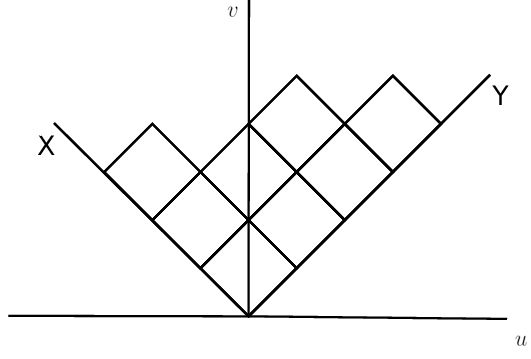
\includegraphics[width=0.6\textwidth]{ydiagru}
    \caption{Russian convention for Young diagrams.}
    \label{fig:ydiagru}
\end{figure}
There are two natural statistics associated to Young diagrams as in \Cref{fig:ydiagru}, which are the size and where the vertex touches the bottom. Define 
\[ V_{\lambda} = \qty(\lambda_1 - \frac{1}{2}) \wedge \qty(\lambda_2 - \frac{3}{2}) \wedge \cdots \]

We now define the operators
\[ \psi_k v = \ul{k} \wedge v. \]
Then we have
\[ :\psi_i \psi_j^*: = \begin{cases}
    \psi_i \psi_j^* & j > 0 \\
    - \psi_j^* \psi_j & j < 0.
\end{cases}
\]
We can check that $[\psi_i, \psi_j] = [\psi_i^*, \psi_j^*] = 0$ and $\psi_i \psi_j^* + \psi_j^* \psi_i = \delta_{ij}$. If we consider $E_{ij} \in \mf{gl}(\infty)$, then assigning $E_{ij} \mapsto \psi_i \psi_j^*$ gives a projective representation of $\mf{gl}(\infty)$. The Casimir operator is $C = \sum_{k \in \Z + \frac{1}{2}} E_{kk}$, and this acts by
\[ C v_S = (\abs{S_+} - \abs{S_-}) v_S. \]
In addition, the operator $H = \sum k E_{kk}$ acts by 
\[ H v_{\lambda} = \abs{\lambda} v_{\lambda}. \]

Define the operators
\[ \mc{E}_r(z) = \sum e^{z(k-r/2)} E_{k-r,k} + \frac{\delta_{r,0}}{\zeta(z)}, \]
where $\zeta(z) = e^{z/2} - e^{-z/2}$. In particular, we have $\mc{E}_r(0) = \sum E_{k-r, k} = \alpha_r$ for $r \neq 0$, where $[\alpha_k, \alpha_r] = k \delta_{k+r}$.

The space $\qty(\bigwedge^{\infty/2} V)_0$ has two natural bases given by the $v_S$ and by $\prod \alpha_{k_i} v_{\emptyset}$. The transition function between them is $\chi_{\mu}^{\lambda}$. This appears in the Gromov-Witten theory of $\P^1$:
\begin{align*} 
    \mel**{\mu}{\prod \tau_{k_i}(\omega)}{v}^{\P^1} &= \frac{1}{\zeta(\mu) \zeta(\lambda)} \sum_{\abs{\lambda} = \abs{\mu}} \chi_{\mu}^{\lambda} \chi_{\nu}^{\lambda} \times \prod \frac{\P_{k_i+1}(\lambda)}{(k_i+1)!} \\ 
    &= \mel**{\alpha_{\mu}}{\prod_{i=1}^n \frac{[z^{k_i}] \mc{E}_0(z)}{k_i!}}{\alpha_{\nu}},
\end{align*}
where the last equality uses the formula $[z^k](\mc{E}_0(z)) v_{\lambda} = \P_k(\lambda) v_{\lambda}$. The last formula we will write in this section is the relation
\[ [\mc{E}_a(z), \mc{E}_b(w)] = \zeta\qty(\det \mqty(z & a \\ w & b)) \mc{E}_{a+b}(z+w). \]

\section{Equivariant Gromov-Witten theory of $\P^1$}

We are interested in an equivariant version of the GW/Hurwitz correspondence, so we want to compute the Gromov-Witten invariants
\begin{align*}
    \braket{a_{k_1}([0]) \cdots a_{k_m}([0])}{\mu}^{\P^1/\infty}_{\C^{\times}} &= \braket{\alpha_{k_1} \cdots \alpha_{k_m} \wt{W}}{\mu} \\
    &= \mel**{\vec{k}}{\wt{W}}{\mu},
\end{align*}
where the $a_{k_i}$ are Getzler descendents, $\wt{W}$ is the operator in~\Cref{thm:op02}, and $\mu$ is ramification data over $\infty$.

\subsection{Localization in Gromov-Witten theory}

Focusing on the case of $\P^1$, we will discuss localization. We begin with the moduli space $\ol{\mc{M}}^{\bullet}_{g, n+m}(\P^1, d)$ of disconnected stable maps, and the fixed points 
\[ \qty(\ol{\mc{M}}_{g, n+m}(\P^1, d))^{\C^{\times}} \] 
with respect to the $\C^{\times}$ action $\xi (v_1, v_2) = (v_1, \xi v_2)$ are simply a moduli space of bipartite graphs with extra markings on the vertices (genuses $g_i$ and marked points) and the edges (degrees $d_{ij}$) subject to various conditions, for example
\[ \sum d_{ij} = d. \]
Then recall that $H^*_{\C^{\times}}(\mr{pt}) = \C[t]$ and $H^*_{\C^{\times}}(\P^1) = \C[h,t]/h(h+t)$. 

In particular, we see that
\[ \qty( \ol{\mc{M}}^{\bullet}(\P^1, d) )^{\C^{\times}} = \bigsqcup_{\vec{g}, \vec{k}} \frac{ \ol{\mc{M}}_{g_1, k_1}, \ol{\mc{M}}_{g_{\ell}, k_{\ell}} }{\Aut}, \]
so we need to consider integrals over this space.

One standard technique is to cut the edges in half and consider the vertices and then glue the edges together, and this puts the markings and the degree $d_{ij}$ copies of $\P^1$ on the same footing. We now need to compute the contribution of a vertex $v_0$ to our integral. We want to compute the contribution of $v_0$ to
\[ \ev{\tau(z_1)[0] \cdots \tau(z_n)[0] \tau(w_1)[\infty]\cdots\tau(w_m)[\infty]}, \]
which is in fact
\[ C^{\circ}(v_0) = \frac{\prod_{i=1}^{e(v_0)} \frac{d_i^{d_i}}{d_i!}}{t^{2g(v_0) - 2 + d(v_0) + \mr{val}(v_0)}} \times H^{\circ}_{g(v_0)(d_1, \ldots, d_{e(v_0)}, \ldots, tz_i, \ldots)}. \]

\subsection{Hodge integrals}

The main component of this computation is the $H^{\circ}$ terms, which are called \textit{Hodge integrals}. Let 
\[\pi \colon C \to \ol{\mc{M}}_{g,n} \] 
be the universal curve on the moduli space of curves. Then 
\[ \mathbb{E} = \pi_*(\omega_{\pi}) \] 
is a rank $g$ vector bundle, called the Hodge bundle. Then let $\lambda_i = c_i(\E)$ be the Hodge classes and $\psi_i = c_1(T^*_{z_i} C)$ be the psi classes. The Hodge integral is now
\[ H^{\circ}_g(z_1, \ldots, z_n) = \prod z_i \int_{\ol{\mc{M}}_{g, n}} \frac{1 - \lambda_1 + \cdots \pm \lambda_g}{\prod_{i=1}^n (1-z_i \psi_i)}. \]

There is a connection between Hodge integrals and Hurwitz numbers in the nonequivariant case, due to Ekedahl-Lando-Schapiro-Vainshtein~\cite{elsv}. The main contribution of Okounkov-Pandharipande~\cite{op2} is to replace the Hurwitz numbers in the equivariant case. First, we consider $C_g(\mu)$, which counts genus $g$ curves with simple ramification at $c_1, \ldots, c_b$ and ramification data $\mu$ at $\infty$, where
\[ b = 2g + \abs{\mu} + \ell(\mu) - 2 \]
by the Riemann-Hurwitz formula. By ELSV, this number is computed by the formula
\[ C_g(\mu) = \frac{b!}{\zeta(\mu)} \qty(\frac{\prod \mu_i^{\mu_i}}{\mu!}) H_g^{\circ}(\mu_1, \ldots, \mu_{\ell}). \]

Our next goal is to interpret $C_g(\mu)$ in the Fock space analytically. Write
\[ \mc{A}(a,b) = S(b)^a \times \sum_{k \in \Z} \frac{\zeta(b)^k}{(a+1)_k} \mc{E}_k(b), \]
where
\[ (a+1)_k = \begin{cases}
    (a+1) \cdots (a+k) & k \geq 0 \\
    (a(a-1)\cdots(a+k+1))^{-1} & k \leq 1
\end{cases}
\]
is the Pochammer symbol. In the case where $m \in \Z$ and $(a,b) = (m, um)$, we obtain
\[ \mc{A}(m, um) = \sum_{n \geq 0} \frac{\zeta(u)^n}{n!} \mc{E}_{n-m}(u). \]
Keeping $b$ as the number of simple branch points, we obtain

\begin{lem}[\cite{op2}]
    We have the identity
    \begin{align*}
        C_g(\mu) &= \frac{b!}{\zeta(\mu)} \qty(\frac{\prod \mu_i^{\mu_i}}{\mu!}) H_g^{\circ}(\mu_1, \ldots, \mu_{\ell}) \\
        &= \ev{\prod_{i=1}^{\ell} \mc{A}(\mu_i, u \mu_i)} \\
        &= \frac{u^?}{\zeta(\mu)} \ev{e^{\alpha_1} \mc{P}_2^b \prod \alpha_{-\mu_i}},
    \end{align*}
    where we use the formula
    \[ \frac{u^m m^m}{m!} \mc{A}(m, um) = e^{\alpha_1} e^{u \mc{P}_2} \alpha_{-m} e^{u \mc{P}_2} e^{-\alpha_1}. \]
\end{lem}

We will also discuss some more properties of the $\mc{A}_{a,b}$. First, there is the identity
\[ [\mc{A}(z, uz), \mc{A}(w, uw)] = \frac{1}{w} \sum_{k \in \Z} \qty(-\frac{z}{w})^k = \delta(z, -w), \]
and second
\[ [u^k] \qty(\prod_{i < j} (z_i + z_j) \times \ev{\mc{A}(z_1, uz_1) \cdots \mc{A}(z_n, uz_n)}) \in \Q[z]. \]

\begin{exm}
    We have an explicit example of a Hodge integral
    \begin{align*}
        H^0(z_1, z_2, u) &= \frac{S(uz_1)^{z_1} S(uz_2)^{z_2}}{\zeta(u(z_1+z_2))} \times \sum_{k > 0} \zeta(ku(z_1+z_2)) \times \frac{\zeta(uz_1)^k \zeta(uz_2)^{-k}}{(1+z_1)_k (1+z_2)_{-k}}
    \end{align*}
    with two insertions.
\end{exm}

\subsection{Application to Gromov-Witten theory}

Returning to the vertex contributions, we obtain
\begin{align*}
    (\cdots) H(d_1, \ldots, d_n, tz_1, \ldots, tz_m) &= (\cdots) \ev{\mc{A}(tz_1, uz_1) \cdots \mc{A}\qty(d_1, \frac{u}{t}d_1) \cdots} \\
    &= (\cdots) \ev{\mc{A}(tz_1, uz_1) \cdots e^{\alpha_1} e^{\frac{u}{t} \mc{P}_2} \prod \alpha_{-d_i}}.
\end{align*}
If we let $P_d$ be the projection operator on $\ker(H-d)$ and write it explicitly as
\[ P_d = \sum \frac{1}{\zeta(\mu)} e^{-\frac{u}{t}} \mc{P}_2 \prod \alpha_{-\mu_i} P_0 \prod \alpha_{\mu_i} e^{-\frac{u}{t} \mc{P}_2}, \]
then we obtain the formula
\begin{align*}
    \ev{\tau(z_1)[0]\cdots\tau(z_n)[0]\tau(w_1)[\infty]\cdots\tau(w_m)[\infty]} &= \sum_{\mu} H(t \vec{z}, \mu) (\cdots) H(-t\vec{w}, \mu) \\
    &= \ev{\prod_{i=1}^n \mc{A}(tz_i, uz_i) e^{\alpha_1} P_d e^{-\alpha_1} \prod_{i=1}^m \mc{A}^*(-t w_i, uw_i)}.
\end{align*}
When $m = 0$, the formula simplifies to
\begin{align*}
    \ev{\tau(z_1)[0]\cdots\tau(z_n)[0]} &= \ev{\prod_{i=1}^n \mc{A}(tz_i, uz_i) e^{\alpha_1} P_d e^{-\alpha_{-1}}} \\
    &= \ev{\prod_{i=1}^n \mc{A}(tz_i, uz_i) \frac{\alpha_1^d}{d!}} \\
    &= \braket{\prod_{i=1}^n \mc{A}(tz_i, uz_i)}{1^d} \\
\end{align*}

\subsection{Dressing operator}

Recall that we want to compute the Gromov-Witten invariants with Getzler descendents, which are given by
\[ \braket{a_{k_1}([0]) \cdots a_{k_n}([0])}{\mu}^{\P^1/\infty, \C^{\times}} = \braket{\alpha_{k_1} \cdots \alpha_{k_n} W e^{\alpha_1}}{\mu}. \]
It remains to describe this matrix $W$ and the variant $\wt{W} = W e^{\alpha_{1}}$. Here, the $a_n$ are defined by
\[ \sum_{n=0}^{\infty} z^n \tau_n = \sum_{n=0}^{\infty} \frac{(iuz)^{n-1}}{1+zc_1} a_n, \]
so for example we have
\[ \tau_1 = \frac{iu}{2} a_2 - c_1 a_1. \]

We will work in $\mf{gl}_{\infty}(V)$. We also write 
\[ \wt{\mf{gl}}(V) = \ev{H^a S^b}_{a,b \in \Z}, \] 
where $H = \sum k E_{kk}$ and $S = \alpha_{-1} = \sum E_{k,k-1}$, so $SH = (H+1)S$. Then define the operator
\[ \wt{\mc{A}} = \frac{1}{u} \sum \frac{(uz)^k}{(tz+1)_k} \alpha_k. \]
Both the operators $\mc{A}, \wt{\mc{A}}$ live in $\mf{gl}(V)[[z^{\pm 1}, u^{\pm 1}, t^{\pm 1}]$. 
Then we will have $W^{-1}AW = \wt{A}$.

\begin{lem}
    Write $D = S^{-1} + H$, $Z = \frac{tS}{u}$, and $\wt{D} = D - \frac{1}{2} \qty(H \frac{1}{1-Z} + \frac{1}{1-Z}H)$. Then there exists a unique solution to the equation
    \[ \dv{W}{t} = WB, \qquad B = \frac{H^2 Z^2}{(1-Z)^2} + \frac{HZ^2}{(1-Z)^3} + \frac{2Z^3 + 3Z^2}{8(1-Z)^4} \]
    such that
    \begin{enumerate}
        \item $W |_{u=0} = 1$;
        \item $W^{-1} DW = \wt{D}$;
        \item $W$ is upper triangular.
    \end{enumerate}
\end{lem}

\begin{proof}[Sketch of proof]
    We will compute the derivative
    \begin{align*}
        \dv{t} (W \wt{D} W^{-1}) &= W \qty(\frac{1}{t} [B, \wt{D}] + \dv{\wt{D}}{t})W^{-1},
    \end{align*}
    and this implies that $\wt{D}|_{t=0} = D|_{t=0}$. Some more ``basic checking'' completes the proof.
\end{proof}

\begin{rmk}
    The operator $B$ in the lemma was discovered by a computer and it is unclear why it appears.
\end{rmk}

\begin{thm}[\cite{gwptdescendent}]
    We have the formula
    \[ W^{-1} \mc{A} W = \wt{\mc{A}}. \]
\end{thm}

\begin{proof}
    Define the operator
    \[ \mc{A}^{(m)} \coloneqq \frac{u^{m+1}m^m}{m!} \mc{A}|_{t=1,z=m} \]
    and define $\wt{\mc{A}}^{(m)}$ analogously. In fact, we have $\mc{A}^{(m)} = (\mc{A}^{(1)})^m$ and
    \begin{align*}
        \wt{\mc{A}}^{(m)} &= S^m e^{\frac{mu}{S}} \\\
        \mc{A}^{(m)} &= e^{\frac{u}{S}} e^{\frac{uH^2}{2}} S^m e^{\frac{-uH^2}{2}}.
    \end{align*}
    Thus we obtain $W^{-1} \mc{A}^{(1)} W = \wt{\mc{A}}^{(1)}$. Differenting both sides by $t$, we obtain the desired result.
\end{proof}

\section{GW/PT correspondence}

Let $X$ be a threefold and consider Pandharipande-Thomas theory on $X$, which we defined in~\Cref{sub:pt}.

\begin{exm}
    Let $X = \P^3$ and $\beta = \P^1$. Then
    \[ P_n(X, \beta) = \qty{L \subset \P^3 \mid n \text{ points on }L}, \]
    and we will call the $n$ points $z_1, \ldots, z_n$. Then we see that
    \[ \mc{O}_{\P^3} \xrightarrow{\varphi} \mc{F} = \mc{O}_L(n) \]
    and $\varphi$ has zeroes at $z_1, \ldots, z_n$. In particular, we have
    \[ \on{vir-dim} P_n(X, \beta) = \dim \mr{Gr}(\P^1, \P^3). \]
    This and similar examples were worked out by Pandharipande-Thomas~\cite{ptthy} and by Moreira~\cite{moreira}.
\end{exm}

\begin{exm}
    Consider $X = \P^1 \times \C^2$. We will consider the moduli space $P_{\chi}(\C^2 \times \P^1, n \P^1)$. If we consider the torus $T_0$ preserving the symplectic form on $\C^2$, then the virtual class satisfies
    \[ [P_{\chi}(\P^1 \times \C^2)]^{\mr{vir}}_{T_0} = \delta_{\chi, n}[\Hilb_n(\C^2)]. \]
\end{exm}

\subsection{Descendents in PT theory}

Let $\F$ be the universal stable pair on $P_n(X, \beta) \times X$. Then if $\gamma \in H^*(X)$, we define
\[ \ch_k(\gamma) = \int_X \ch_k(\F - \mc{O}) \cdot \gamma. \]
When $X = \P^1 \times \C^2$, then 
\[ \int_{P_n(X, n \P^1)} \prod_{i=1}^n \ch_{k_i}(\gamma_i) = \int_{\Hilb_n(\C^2)} \prod \ch_{k_i}(\gamma_i). \]
Then there is the formula
\[ \ch(z)([0]) \ket{[I_{\lambda}]} = S^{-1} \qty(\frac{x}{s})e^{zH} \ket{v_{\lambda}}. \]
Of course, if $\C^{\times}$ acts on $\C^2$ with the antidiagonal action, we see that
\[ (\Hilb_n(\C^2))^{\C^{\times}} = \bigsqcup_{\abs{\lambda} = n} \qty{I_{\lambda}}, \]
where $I_{\lambda} = (x^{\lambda_1}, x^{\lambda_2}y, \ldots, x^{\lambda_{\ell}} y^{\ell})$. Then we have $\mc{O} / I_{\lambda} = \mc{F}$, and so
\begin{align*} 
    \ch(\mc{F}) |_{I_{\lambda}} &= \sum_{ij \in \lambda} e^{s(i-j)} \\ 
    &= \sum_{i=1}^{\ell} \frac{e^{(\lambda_i - i)s}-1}{e^s-1}.
\end{align*}
The $S^{-1}\qty(\frac{x}{s})$ term comes from the presence of the Todd class. Recall the definition
\begin{align*}
    H^{\mr{PT}}(x) &= \sum_{k=-1}^{\infty} x^{k+1} H_k^{\mr{PT}} \\
    &= S^{-1}\qty(\frac{x}{\theta}) \sum_{k=0}^{\infty} x^k \ch_k(\F-\mc{O}),
\end{align*}
where $\theta^{-1} = -c_2(T_X)$.

Now the main formula is that for $s=1$, we have
\begin{align*} 
    \mel**{1^n}{\prod_{i=1}^n H_{k_i}^{\mr{PT}}([0])}{\mu}^{T_0} &= [z^{\vec{k}}] \mel**{e^{\alpha_1}}{e^{\qty(\sum z_i)H}}{\mu} \\
    &= [z^{\vec{k}}]\braket{e^{\qty(\sum z_i)(H+\alpha_1)}e^{\alpha_1}}{\mu} \\
    &= [z^{\vec{k}}] \braket{W^{-1} e^{\qty(\sum z_i) D}e^{\alpha_1}}{\mu} \\
    &= [z^k] \braket{e^{\qty(\sum z_i)\wt{D}}We^{\alpha_1}}{\mu}.
\end{align*}
On the Gromov-Witten side, we have
\begin{align*}
    \mel**{1^n}{\prod_{i=1}^n H_{k_i}^{\mr{GW}}([0])}{\mu} = \braket{\prod \alpha_{k_i}W^{-1}e^{\alpha_1}}{\mu}.
\end{align*}
This allows us to solve the GW/PT correspondence and match descendents, where
\begin{align*}
    e^{z\wt{D}} &= \ch(z)[0] \\
    \alpha_k &= \tau_k([0]).
\end{align*}
This actually allows us to define negative descendents, but to match the descendents we need to write $\wt{D}$ in terms of the $\alpha_k$.

\subsection{Matching GW and PT descendents}

Our method will be to do the following:
\begin{enumerate}
    \item Diagonalize $D$;
    \item If $A \in \mf{gl}(V)$ is diagonal with eigenvalues
        \[ A \ul{\qty(k+\frac{1}{2})} = \lambda_k \ul{\qty(k+\frac{1}{2})}, \]
        then $A$ acts on $\bigwedge^{\infty/2} V$ by
        \[ \Res_{w=0} \qty(\sum_{k \in \Z} \lambda_k w^{-k}) \times \psi(w) \psi^*(w). \]
        There is a boson/fermion correspondence between
        \begin{align*}
            \psi(x) &= T x^{c+\frac{1}{2}} \Gamma_+(x), \\
            \psi^*(x) &= T^{-1} x^{-c+\frac{1}{2}} \Gamma_-(x).
        \end{align*}
\end{enumerate}

The first step is of course to diagonalize $D$ (for simplicity, we will set $t=s=1$). Clearly we can identify
\[ V = z^{\frac{1}{2}} \C[z][[z^{-1}]]. \]
Then we know
\[ D = \qty(\frac{1}{z} - \dv{z} \frac{z^2}{(iu-z)} - \frac{1}{2} \frac{z}{(1-z)^2}) f(z), \]
so we need to solve the differential equation $Df(z) = \lambda f(z)$. The solution is
\[ f(z) = \qty(1-\frac{z}{iu})^{-\frac{1}{2}} z^{\frac{1}{2}-\lambda} \times \exp \qty[\frac{iu}{2z^2} - \frac{(1+iu\lambda)}{z}]. \]
To make this work, we need $\lambda \in \Z$, and to diagonalize $D$ we take the basis
\[ f_k(z) = \qty(z^{-1} e^{\frac{-iu}{z}})^k \times \exp(g(z)), \]
where $g(z) = -\frac{iu}{2z^2} + \frac{1}{z} - \frac{1}{2} \log\qty(1-\frac{iu}{z})$. The Lambert curve is obtained from $f_k$, which produces the curve 
\[ xe^{-x} = ye^{-y} e^{\frac{x}{\theta}}. \]

\begin{rmk}
    Recall the dressing operator $W$, which we defined using a differential equation. An explicit formula for $W$ is
    \[ W = W_{\lambda,\mu} = \braket{a_{\lambda}}{\mu}^{\P^1, \C^{\times}}. \]
\end{rmk}

An upgraded version of the GW/PT correspondence is the following:
\begin{thm}[\cite{gwptdescendent}]
    Subject to $t_1 + t_2 = 0$, there is an explicit equality of descendent vertices
    \[ \braket{\prod H_{k_i}^{\mr{GW}}([0])}{\emptyset, \emptyset, \mu}^{\mr{GW}, T_0} =\braket{\prod H_{k_i}^{\mr{PT}}([0])}{\emptyset, \emptyset, \mu}^{\mr{PT}, T_0}. \]
\end{thm}

\begin{rmk}
    Using the Pandharipande-Pixton philosophy, we can obtain equality~\Cref{thm:oopmain}. This will be enough to prove the stationary GW/PT correspondence for toric varieties.
\end{rmk}

\subsection{GW/PT correspondence with descendents}

Recall that on the Gromov-Witten side, the insertions of interest are $\tau_0(\gamma)$, while in PT theory, the corresponding insertions should be $\ch_2(\gamma)$. This correspondence was proved in~\cite{moop} for any toric variety and any $\gamma$, while Pandharipande-Pixton~\cite{ppquintic} prove this for $X$ a complete intersection in $\P^N$. There is also a conjectural equality between $\tau_k([\mr{pt}])$ and $\ch_{k+2}([\mr{pt}])$.

More generally,~\cite{mnop2} conjecture that there is a series of ``chemical reactions'' that take
$\prod_{i=1}^n \tau_{k_i}(\gamma_i)$ to an expression involving with Chern classes.

Pandharipande-Pixton~\cite{ppgwptdesc} consider the operators
\begin{align*}
    M_{\lambda,\mu}^{\mr{PT}} = \braket{\prod \ch_{\lambda_i + 2}([0])}{\mu}_{\mr{PT},T}^{\C^2 \times \P^1 / \C^2 \times \infty} \\
    M_{\lambda,\mu}^{\mr{GW}} = \braket{\prod \tau{\lambda_i}([0])}{\mu}_{\mr{GW}, T}^{\C^2 \times \P^1 / \C^2 \times \infty}
\end{align*}
in the fully equivariant case. This fits into an overall picture
\begin{equation*}
\begin{tikzcd}
    \text{GW desc} \ar{r}{M^{\mr{GW}}} & \text{rel conds} & \text{PT desc} \ar[swap]{l}{M^{\mr{PT}}} \ar[bend left=30]{ll}{M^{\mr{GW/PT}} = M^{\mr{GW}} \circ (M^{\mr{PT}})^{-1}}.
\end{tikzcd}
\end{equation*}

\begin{thm}[\cite{ppgwptdesc}]\leavevmode
    \begin{itemize}
        \item The operator $M^{\mr{PT}}$ is rational in $q$;
        \item The operators $M^{\mr{PT}}$ and $M^{\mr{GW}}$ are upper-triangular.
        \item There is an equality
            \[ \ev{M^{\mr{GW/PT}}(D)}_{\mr{GW},T}^X = \ev{D}_{\mr{PT},T}^X \]
            for any $X$ and any $D = \prod_{i=1}^m \ch_{k_i}(\gamma_i)$.
    \end{itemize}
\end{thm}

While $M^{\mr{GW/PT}}$ is unknown, there is an explicit formula for some of the matrix elements, which we call $C^{\bullet}$.
\begin{thm}[\cite{gwptdescendent}]
    There is an explicit equality
    \[ \ev{C^{\bullet}\qty(\prod_{i=1}^n \ch_{k_i}(\gamma_i))}_X^{\mr{GW}} = \ev{\prod \ch_{k_i}(\gamma_i)}_X^{\mr{PT}} \]
    for any toric $X$ and stationary descendents $\gamma_i \in H^{>0}(X)$.
\end{thm}

We will consider the formal algebras
\begin{align*}
    \mathbb{D}_{\mr{PT}}^X &\supset \mathbb{D}_{\mr{PT}}^{ X, \mt{st} } \coloneqq \braket{\ch_i(\gamma) \mid i \geq 2, \gamma \in H^{>0}} \\
    \mathbb{D}_{\mr{GW}}^X &\supset \mathbb{D}_{\mr{GW}}^{ X, \mt{st} } \coloneqq \braket{\tau_i(\gamma) \mid i \geq 0, \gamma \in H^{>0}}.
\end{align*}
Then write
\[ \wt{\ch}_k(\gamma) \coloneqq \ch_k(\gamma) + \frac{1}{24} \ch_{k-2}(\gamma \cdot c_2). \]
Then we can write
\[ C^{\bullet}\qty(\prod_{i=1}^m \wt{\ch}_i(\gamma)) = \prod_{P \text{ partition of } (1, \ldots, n)} \prod_{s \in P} C^{\circ} \qty(\prod_{s \in P} \wt{\ch}_{{k_i}}(\gamma_i)). \]
The $C^{\circ}$ are quite complicated, but in a simple case, we have
\[ C^{\circ}(\wt{\ch}_{k_1+2}(\gamma) \wt{\ch}_{k_2 + 2}(\gamma')) = -\frac{(iu)}{k_1!}{k_2!} a_{k_1+k_2}(\gamma \cdot \gamma') + \sum (*) a_{\mu_1} a_{\mu_2}(\gamma \cdot \gamma' c_1). \]
There is a bumping and splitting that produces things like
\[ a_k a_{\ell}(\alpha) = \sum_{i=1}^N a_k(\alpha_i^L) a_{\ell}(\alpha_i^R), \]
where $\Delta \cdot \alpha = \sum \alpha_i^L \otimes \alpha_i^R \in H^*(X \times X)$. We will take the $\alpha_i^L$ and $\alpha_i^R$ to have degrees $d^L, d^R$, respectively.

\subsection{Virasoro constraints in PT theory}

For a toric variety $X$, we can apply the GW/PT correspondence to the Virasoro constraints for $\mr{GW}(X)$. This obtains Virasoro constraints for $\mr{PT}(X)$, which turns out to be quite simple. The Virasoro constraints in PT theory are:
\begin{itemize}
    \item We have
        \[ R_k(\ch_i(\gamma)) = \qty(\prod_{n=0}^k (i+d-3+n)) \ch_{i+k}(\gamma) \]
        for any $\gamma \in H^{2d}(X, \Q)$. For example, $R_{-1}(\ch_i(\gamma)) = \ch_{i=1}(\gamma)$.
    \item The constant terms are
        \begin{align*} 
            T_k ={}& -\frac{1}{2} \sum_{a+b=k+2} (-1)^{d^L d^R}(a+d^L-3)!(b+d^R-3)! \ch_a \ch_b(c_1) \\ 
            &+ \frac{1}{24} \sum_{a+b=k} a! b! \ch_a \ch_b(c_1 c_2). 
        \end{align*}
    \item There are also the operators $L_k^{\mr{PT}} = T_k + R_k$ satisfying
        \[ L_k^{\mr{PT}}, L_{\ell}^{\mr{PT}} = (k+\ell) L_{k+\ell}^{\mr{PT}} \]
        and operators $\mc{L}_k^{\mr{PT}} = L_k^{\mr{PT}} + (k+1)! L_{-1}^{\mr{PT}} \ch_{k+1}(p)$.
\end{itemize}

\begin{thm}[\cite{virasoropt}]
    For any $D \in \mathbb{D}^{\mr{PT},\mr{st}}$, we have
    \[ \ev{\mc{L}_k^{\mr{PT}}(D)}_X^{\mr{PT}} = 0. \]
\end{thm}

\begin{conj}
    The theorem holds for all descendents $D \in \mathbb{D}^{\mr{PT}}$.
\end{conj}

The proof essentially amounts to checking the following formula:
\begin{thm}
    There is the formula
    \[ C^{\bullet} \circ L_k^{\mr{PT}}(D) = (iu)^{-k} \wt{\mc{L}}_k^{\mr{GW}} \circ C^{\bullet}(D). \]
\end{thm}
Here, $L_k^{\mr{GW}}$ is the usual Virasoro for Gromov-Witten theory.\footnote{Alexei complained about this not preserving stationary things.} The only contribution to descendents of $1$ to $L_k^{\mr{GW}}$ are
\[ (k+1)! \tau_0(1) \tau_{k-1}(p) = T_k^{\circ}. \]
Therefore, we can define $\wt{L}_k^{\mr{GW}} = L_k^{\mr{GW}} - T_k^{\circ}$ and $\mc{L}_k^{\mr{GW}} = \wt{\mc{L}}_k^{\mr{GW}} + (iu)^2 (k+1)! \wt{L}_{-1}^{\mr{GW}}$.
\begin{prop}\leavevmode
    \begin{itemize}
        \item The operator $\mc{L}_k^{\mr{GW}}$ preserve stationary descendents, as in
            \[ \mc{L}_k^{\mr{GW}}(\mathbb{D}^{\mr{GW}, \mr{st}}) \subset \mathbb{D}^{\mr{GW}, \mr{st}}. \]
        \item We have the vanishing
            \[ \ev{\mc{L}_k^{\mr{GW}}(D)}^{\mr{GW}} = 0 \]
            for all $D \in \mathbb{D}^{\mr{GW}}$.
    \end{itemize}
\end{prop}

Let $S$ be a surface and $X = S \times \P^1$. Then
\[ P_n(S \times \P^1, [n \P^1]) = \Hilb_n(S), \]
and so the virtual class is
\[ [P_n(S \times \P^1, [n \P^1])]^{\mr{vir}} = [\Hilb_n(S)]. \]
Then if $\mc{I}$ is the universal ideal on the Hilbert scheme, define
\[ \ch_k^{\Hilb}(\gamma) = \int_S \ch_k(\mc{I}) \gamma. \]
\begin{cor}
    For any toric surface $S$ and $\gamma_i \in H^*(S)$, we have
    \[ \int_{\Hilb_n(S)} \mc{L}_k^{\Hilb} \qty(\prod_{i=1}^n \ch_{k_i}^{\Hilb}(\gamma_i)) = 0. \]
\end{cor}

\begin{proof}
    This follows from
    \[ \ch_{k_i}(\gamma \times [\mr{pt}]) = \ch_{k_i}^{\Hilb}(\gamma). \]
\end{proof}

\begin{rmk}
A cobordism argument was used by Moreira~\cite{moreira} to extend this to any surface $S$ with $H^1(S) = 0$.
\end{rmk}


\chapter{Counting curves in 1, 3, \xout{and 5} dimensions (Andrei Okounkov)}%
\label{cha:andrei}

The main object in Gromov-Witten theory is the moduli space $\mc{M}_{\mr{GW}}$ of stable maps $C \to X$ from a curve to $X$. This is of course highly disconnected, so the genus $g$ component will be weighted by $u^{2g-2}$ while we will hide the degree component for now. One of the major ideas in this subject is to push forward cohomology classes to the moduli of curves, which forms a \textit{cohomological field theory} with rich structure coming from maps between different moduli spaces of curves. Instead, we will push things forward to $X$. Just like we can vary the source curves in families, we can degenerate $X$. Also, automorphisms of $X$ still act on our moduli space.

Our goal is to give a target space description of integrals over $\mc{M}_{\mr{GW}}$. We would like a geometric theory that reproduces the same integrals and an algebraic theory that computes them in some fashion resembling a topological quantum field theory -- for example Chern-Simons theory.

\begin{figure}[h]
    \centering
    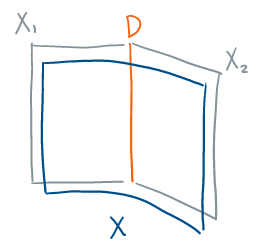
\includegraphics[width=0.4\textwidth]{basicdeg}
    \caption{Basic degeneration}
    \label{fig:basicdeg}
\end{figure}

The most basic degeneration of a variety $X$ is to degenerate 
\[ X \rightsquigarrow X_1 \cup_D X_2, \] 
where $D$ is a smooth divisor shared between $X_1$ and $X_2$ as in~\Cref{fig:basicdeg}. If we write $\P = \P(\mc{O}_D \oplus N_{X_i/D})$, we obtain the relation
\[ [X] = [X_1] + [X_2] - [\P] \]
in algebraic cobordism. As proved by Levine-Pandharipande~\cite{algcob}, this relation generates all relations in algebraic cobordism. A similar type of degeneration is the expanded degeneration of Jun Li~\cite{expdeg}, which creates an accordion of $\P^1$-bundles as in~\Cref{fig:extdeg}.

\begin{figure}[h]
    \centering
    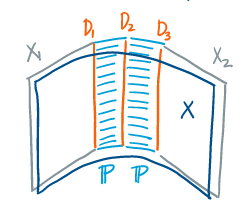
\includegraphics[width=0.4\textwidth]{extdeg}
    \caption{Expanded degeneration}
    \label{fig:extdeg}
\end{figure}

This fits well into the usual TQFT formalism where the boundary divisor $D = \bigsqcup D_i$ is associated to a vector space $\mc{H}(D) = \bigotimes \mc{H}(D_i)$ and the manifold $X$ is a vector in this space. Because $\mc{H}(D)$ is usually the cohomology of some nice space, it has a product $\cup$, integration, and a form
\[ (\alpha, \beta) = \int \alpha \cup \beta. \]
We can impose conditions at $D$ by either pulling back cohomology classes from $D$ or pushing forward to a cohomology class in $\mc{H}(D)$.

In reality, we have more general degenerations, where we have a degeneration
\[ X \rightsquigarrow \bigcup_i X_i, \]
where the $X_i$ are glued along a simple normal crossings divisor. This has been extensively studied in geometry, for example in logarithmic Gromov-Witten theory, logarithmic Donaldson-Thomas theory of Maulik-Ranganathan~\cite{logdt}, and Brett Parker's ``exploded manifolds''~\cite{expman}.

\section{Counting curves in 1 dimension}

Now, we will take $\dim X = 1$, so we are studying maps $f \colon C \to X$ from a curve. We can take $X = \P^1$ or even $X = \C$ with the action of $\C^{\times}$. Before we begin, we would like to discuss why we prefer $\dim X$ to be odd. If we consider $X \times \C$, then
\[ [\mc{M}_{\mr{GW}}(X \times \C)]^{\mr{vir}} = [\mc{M}_{\mr{GW}}(X)]^{\mr{vir}} \cup \mr{Eu}(H^1(C, \mc{O}_C) \otimes \C) \ep^{-1}, \] 
where $\ep \in H^2([\mr{pt}/\C^{\times}])$ is a coordinate on $\on{\ms{Lie}} \C^{\times}$. This can be removed by taking $\ep \to \infty$, but doing so is very hard and introduces new problems. However, Mumford tells us
\[ \mr{Eu}(\ep) \otimes \mr{Eu}(-\ep) = (-1)^g \ep^{2g}, \]
and thus changing dimension by $2$ is very easy.

In the case of $\dim X = 1$, the geometric target space theory is just Hurwitz theory, which as in~\Cref{sub:hurwitz} counts ramified covers of $X$ of degree $d$ with specified ramification data. This ramification data is an instance of a relative condition in Gromov-Witten theory, which is as follows. We can consider the moduli space of relative stable maps $\mc{M}_{\mr{GW}}(X/D)$, where we impose that $f^{-1}(D) = \sum \mu_i p_i$, where $\mu$ is a partition and the $p_i$ are the marked points of $C$.

Hurwitz theory has moduli spaces parameterizing maps $C \to X$ which are ramified covers with the specified ramification, where $(X, x_1, \ldots, x_n)$ can vary in moduli. These moduli spaces are finite over the moduli of curves, so the most interesting number is simply the degree of this map, which is the Hurwitz number. Under degenerations $X \rightsquigarrow X_1 \cup X_2$, then the ramification at the node $x_0$ should match. These are called admissible covers; see Harris-Morrison~\cite{harmor} for a reference. This gives us the relation
\[ \mr{Hur}(X, \mu_1, \mu_2, \ldots) = \mr{Hur}(X_1, \mu_1, \ldots, \bullet) \cdot \mr{Hur}(X_2, \mu_2, \ldots, \bullet), \]
where $\bullet = \sum_{\eta} \zeta(\eta) \eta \otimes \eta \in \mc{H} \otimes \mc{H}$. This insertion is inverse to the the pairing on $\mc{H}$.

The general answer for Hurwitz numbers was known to Frobenius and Burnside as
\[ \mr{Hur}(\mu^{(1)}, \mu^{(2)}, \ldots)_X = \sum_{\lambda \in \mr{Irr}(S(d))} \qty(\frac{\dim \lambda}{\abs{S(d)}})^{2-2g} \prod_i (\text{central character of }\mu^{(i)}\text{ in }\lambda). \]
This contains a blueprint for the modern understanding of all 2d TQFTs as well as handle-gluing operators.

\subsection{More algebraic way to think about characters of $S(d)$}

There is the action of a central extension of $\mf{gl}(\infty)$ on $\bigwedge^{\infty/2} \C^{\infty}$, known as the \textit{Fock space}. We need the operators $\psi_k, \psi_k^*$ defined in \Cref{sub:fock}, but we also want the Heisenberg operators
\[ \alpha_n = \sum_{j-i=n} E_{ij}, \]
which act on the vacuum $v_{\emptyset}$ by
\[ \prod \alpha_{-\mu_i} \ket{v_{\emptyset}} = \sum_{\lambda} \chi_{\mu}^{\lambda} \ket{\lambda}. \]

We also want co consider the fermionic operators
\[ P_m = \sum_k k^m \psi_k \psi_k^* \]
taken without the normal ordering and $\zeta$-regularized as in
\[ \sum_{i=1}^{\infty} \qty(-i + \frac{1}{2})^m = (1-2^{-m})\zeta(-m). \]
The operator $P_m$ acts with eigenvalue
\[ p_m(\lambda) = \sum_i \qty(\lambda_i - i + \frac{1}{2})^m \]
on $\ket{\lambda}$. By Vershik-Kerov and Kerov-Olshanski, the central character of $\mu$ and $\lambda$ are polynomials of $\lambda$, which are $\C[p_1, p_2, \ldots]$ and in fact is equal to
\[ \frac{1}{\prod \mu_i} \prod p_{\mu_i} + \cdots, \]
where the lower order terms are controlled by the Gromov-Witten/Hurwitz correspondence. In particular, there is the remarkable formula
\[ \sum z^{d-\frac{1}{24}} \mr{Hur}(\P^1, \mu_1, \ldots) = \mel**{v_{\emptyset}}{e^{\alpha_1} z^{p_1} (\text{fermionic operators}) e^{\alpha_{-1}}}{v_{\emptyset}}, \]
while the case of the elliptic curve is simply the trace of the middle operator without the $e^{\alpha_1}$ terms.

\subsection{Gromov-Witten/Hurwitz correspondence}

There are several features of this correspondence:
\begin{enumerate}
    \item There are no descendents of $1 \in H^0(X, \Q)$ or $H^1(X, \Q)$ in Hurwitz theory. In Gromov-Witten theory, these can be explicitly reduced to descendents of $\mr{pt} \in H^2(X, \Q)$.
    \item Relative conditions correspond to relative conditions. This will always be true in the things that we study.
    \item Descendents of $\mr{pt} \in H^2(X, \Q)$ are equal to relative conditions glued on a $\P^1$ bubble.
\end{enumerate}
This reduces to computing everything in the Gromov-Witten theory of $X = (\P^1, 0, \infty)$, where one of the marked points is descendent and the other is relative.

The remarkable formula in~\Cref{thm:op01} can be computed explicitly and gives a formula for the completed cycles as conjugacy classes. More generally, if we have two relative points, the invariants can be computed explicitly and are B/C-symmetric in $\eta \cup \eta'$. In particular, for $d = 0$, we have
\[ \tau_k(\mr{pt}) v_{\emptyset} = \frac{1}{(k+1)!}(1-2^{-k-1}) \zeta(-k-1), \]
and this was computed by Faber and Pandharipande~\cite{gwhodge}.

We now want to consider the equivariant theory for $\P^1$.
\begin{thm}[\cite{op2}]\label{thm:op02}
    We have the identity
    \[ \braket{\exp\qty(\sum_{i \geq 0} t_i \tau_i([0]))}{\mu} = \braket{\exp\qty(\sum_{n \geq 1} \wt{t}_n \alpha_n) \wt{W}}{\mu}, \]
    where we take a linear change of times determined by
    \[ \sum_{k \geq 0} x^{k+1} \tau_k([0]) \rightsquigarrow \sum_{n \geq 1} \frac{u^{n-1}x^n}{(1+\ep x) \cdots (n+\ep x)} \alpha_n. \]
\end{thm}

\subsection{Role of integrable systems}

This last formula was found by Getzler~\cite{getz} and is problematic in the $\ep \to \infty$ limit. Morally, the Gromov-Witten descendents give a quantum integrable system that looks like a free boson or free fermion. By the Kyoto school of integrable systems, there is a classical integrable system for generating functions. In particular, for $\P^1$ with two marked points, the degeneration gives us
\[ \ev{\exp \qty(\sum_{n \geq 1} \wt{t}_n \alpha_n) g \exp\qty(\sum_{n \geq 1} \wt{s}_n \alpha_{-n})}, \]
which is a tau function for the 2-Toda hierarchy and in particular gives a KP hierarchy for linear Hodge integrals in degree $0$.

\begin{rmk}
    These equations differ from the equations found in 2009 by Kazarian~\cite{kaz}, and this is not well-understood.
\end{rmk}

Fundamentally, these equations come from Pl\"ucker relations for $GL(\infty) \hookrightarrow \End(\mr{Fock})$. This is because in $\mr{Fock} \otimes \mr{Fock}$ there is an invariant operator $\sum \psi_k \otimes \psi_k^*$ commuting with $GL(\infty)$. Our goal now is to understand the deformation of the following for $\dim X = 3$:
\begin{enumerate}
    \item The group $GL(\infty)$;
    \item The representation $GL(\infty) \to \End(\mr{Fock})$;
    \item The quantum integrable system;
    \item The invariant operator in $\mr{Fock} \otimes \mr{Fock}$.
\end{enumerate}

\section{Counting curves in 3 dimensions}

Again, we are looking for a target space description of enumerative theories, but this time for threefolds. Here, we will consider Donaldson-Thomas (sheaf-counting) theories on a threefold $X$. The connection to Gromov-Witten theory was conjectured by Maulik-Nekrasov-Okounkov-Pandharipande~\cite{mnop1,mnop2} building on the work of Aganagic-Klemm-Marino-Vafa~\cite{vertexphys} and the connection to box counting by Okounkov-Reshetikhin-Vafa~\cite{crystals}.

\subsection{Donaldson-Thomas theory}

While Gromov-Witten theory thinks of a curve inside $X$ as a map $f \colon C \to X$, Donaldson-Thomas theory thinks of $C$ as being cut out by the ideal sheaf
\[ \mc{I}_C \in \Hilb(X, \mr{curves}), \]
which has discrete invariants the degree $\beta \in H_2(X, \Z)$ and the holomorphic Euler characteristic $\chi(\mc{O}_C)$. This has a natural obstruction theory
\[ \Ext^i(\mc{I}_C, \mc{O}_C), \]
which is unsuitable for our purposes. Instead, we interpret $\mc{I}_C$ as a rank $1$ torsion-free sheaf with 
\[ \det \mc{I}_C = \mc{O}_C, \]
and so we obtain the obstruction theory
\[ \mr{Def} = \Ext_0^1(\mc{I}_C, \mc{I}_C), \qquad \mr{Obs} = \Ext_0^2(\mc{I}_C, \mc{I}_C). \]
There are no higher Ext groups (even for orbifolds) by a result of Zhou~\cite{relorbdt}.

In Donaldson-Thomas theory, the descendents are $\ch(\mf{I}_C)$, where $\mf{I}_C$ is the universal sheaf on $X \times \Hilb(X)$. We would hope that counts in fixed degree (this does work) and fixed genus (this does not work because moduli spaces are empty for $g \ll 0$ or $\chi \ll 0$) may be related, but unfortinately this is too naive. Instead, we expect a GW/DT correspondence
\[ \sum u^{2g-2} (\cdots) \xleftrightarrow{\text{corresponds}} \sum (-z)^{\chi} (\cdots) \]
after the standard change of variables
\[ z = -e^{iu}, \]
where $z$ is weighted by $\chi$ and $u$ is weighted by genus.

All moduli spaces in Donaldson-Thomas theory are schemes, so all DT invariants are actually integers. If we want actual equality of analytic functions with the Gromov-Witten partition function, we must have rationality of the DT partition function (this is related to BPS integrality). For this all to work out, the virtual dimensions
\begin{align*}
    \mr{GW-vir-dim} &= (\deg, c_1(X)) + (g-1)(3-\dim X) \\
    \mr{DT-vir-dim} &= (\deg, c_1(X))
\end{align*}
must be the same, so $X$ must be a threefold. Of course, our correspondence requires
\begin{enumerate}
    \item Identification of descendents;
    \item Division by degree $0$ contributions in DT theory;
    \item Prefactors like $z^{-\frac{\mr{vir-dim}}{2}} \leftrightarrow (-iu)^{\mr{vir-dim}}$.
\end{enumerate}
See~\cite{takagidt} for precise formulas and additional discussion.

In DT theory, it is possible to remove the degree $0$ terms \textbf{geometrically} using Pandharipande-Thomas theory, which was discussed in~\Cref{sub:pt}. Some parts of identifying the descendents are easy (for example primary descendents and relative conditions are fine). 

\subsection{Relative conditions in DT theory}

In Gromov-Witten theory, a relative condition for a divisor $D$ consists of specifying a condition like 
\[ f^{-1}(D) = 2p_1 + p_2 + 2 p_3. \] 
If $p_2$ and $p_3$ are mapped to the same point with $p_3$ tangent to $D$, then we have an evaluation map to the inertia stack of $S^n D \ni 2 f(p_1) + 3 f(p_2)$, where we remember the ramification data $(2,1)$ on $f(p_2) = f(p_3)$. Therefore, we are really integrating orbifold cohomology classes, where classes in $H^*(D)$ are colored by integers, so we are considering
\[ S^{\bullet} (H^{\bullet}(D) \otimes t \C[t]). \]
If we want to resolve the tangency, then we must degenerate $X$ in a family and bubble off of $\P^1$-bundle on $D$ (or a whole accordion).

In Donaldson-Thomas theory, we have a map
\[ \mc{O}_C(-D) \to \mc{O}_C \to \mc{O}_{C \cap D} \in \Hilb(D, m), \]
which is regular as long as multiplying by the equation of $D$ is injective. To ensure this, we must bubble out the accordion as above. Therefore, the relative conditions come from $H^*(\Hilb(D, n))$, which has a Nakajima basis
\[ \prod \alpha_{-m_i}(\gamma_i) \ket{\mr{vac}}, \]
where the vacuum vector is $1 \in H^0(\Hilb(D, 0))$. Of course, there is an isomorphism
\[ \bigoplus_n H^*(\Hilb(D, n)) \simeq S^{\bullet}(H^*(D) \otimes t \C[t]), \]
and so adding a subscheme of length $m_i$ along $\gamma_i \in H^*(D)$ should correspond to tangency of order $m_i$ along $\gamma_i$.

The GW/DT correspondence has been proved for many, but not all, threefolds, and a key step, as in Maulik-Oblomkov-Okounkov-Pandharipande~\cite{moop}, is to consider a fibration
\[ A_r \hookrightarrow X \to B, \]
where $A_r$ is a crepant resolution of $\C^2/\mu_{r+1}$, where $\mu_{r+1}$ acts with weights $(1, -1)$. Thus $X$ is a crepant resolution of 
\[ \qty(\mc{L}_1 \oplus \mc{L}_2 \to B) / \mu_{r+1}. \]
When $r = 0$, then $X = \mc{L}_1 \oplus \mc{L}_2 \to B$ is a local curve, so for example $B \times \C \times \C$ is fine, and we should recover Hurwitz theory for $\ep_1 + \ep_2 = 0$.

\begin{rmk}
    ADE surfaces are special for many reasons, for example enhanced symmetries of $H^*(\Hilb)$ or of $D^b \ms{Coh}$.
\end{rmk}

The torus fixed points on $\Hilb(B \times \C^2)$ are those curves supported on $B$, which can be thought of having a partition on $B$ (corresponding to the closure of the generic point) with some extra boxes. The DT analog of the Mumford relations is that if $\ep_1 + \ep_2 = 0$, then the virtual class vanishes for all nonminimal cases. Of course, the fixed points of $\Hilb(\C^2, n)$ correspond to partitions. If $\abs{\lambda} = n$, then
\[ T_{\lambda} \Hilb(\C^2, n) = \sum_{\square} (a(\square) + 1) \ep_1 - \ell(\square) \ep_2 + (\ell(\square) + 1) \ep_1 - a(\square) \ep_2, \]
where $a(\square), \ell(\square)$ are the arm and leg lengths respectively. Then we obtain
\[ \Ext^{\bullet}_{X, \circ} (\mc{I}_{\lambda}, \mc{I}_{\lambda}) = H^*(B, -), \]
and so the virtual class is
\[ \prod_{\square} \qty((a+1-\ell)(\ell+1-a))^{2g(B)-2}. \]
When $\ep_1 + \ep_2 = 0$, this becomes
\[ (-1)^{n(1-g(b))} \ep_1^{2n(1-g(b))} \prod_{\square} h(\square)^{2g(B)-2}. \]
This clearly is related to the representation theory of the symmetric group.

\begin{rmk}
    Subsequent to~\cite{moop}, a different perspective was developed, in particular for computations in K-theory. Unfortunately, we cannot say anything about a possible relation to Gromov-Witten theory.
\end{rmk}

\subsection{Role of quantum groups}

If we return to our $A_r$-bundle over $B$, we want some kind of cohomological field theory on the stack of $(\C^{\times})^2$-bundles on curves $B$ (which can vary in moduli). This has various building blocks related to $B = \P^1$ with a descendent at $0$ and relative condition at $\infty$ with the $\C^{\times}$ action. The descendent conditions correspond to
\[ S^{\bullet}(H^*(A_r) \otimes t \C[t]), \]
while the relative conditions correspond to 
\[ H^{\bullet}(\Hilb(A_r)). \]
By the ideas of Nekrasov-Shatashvili~\cite{nekshat}, this structure should be described by a quantum group, and this idea has been realized (also in K-theory) with the quantum group $\mc{U}_{\hslash}\qty(\wh{\wh{\mf{gl}(r+1)}})$ in K-theory and the Yangian for cohomology. Here, if $t_1, t_2$ are the weights of $(\C^{\times})^2$ acting on $\C^2$, then $\hslash = \frac{1}{t_1 t_2}$ is the weight of the symplectic form. There is a noticeable difference between $\mf{gl}$ and $\mf{sl}$, and it becomes more dramatic for other quivers.

\begin{rmk}
    In order to work with these objects, it is important to use a computer, and we would like to advertise the code written by Henry Liu: \url{https://github.com/liu-henry-hl/boxcounting}.
\end{rmk}

\begin{rmk}
    If we restrict to $\ep_1 + \ep_2 = 0$, then
    \[ \ms{Y}(\wh{\mf{gl}(1)}) \simeq \mc{U}(\mf{gl}(\infty)) \]
    as a Hopf algebra, so we recover our description of Hurwitz theory.
\end{rmk}

\begin{exm}
    Recall that the operators corresponding to $\P^1$ with one descendent and two relative conditions commute. These should be Baxter $Q$-operators, and this is more or less true.
\end{exm}

\subsection{Quantum loop algebra}

The \textit{quantum loop algebra} $\mc{U}_{\hslash}(\wh{g})$ is a Hopf algebra deformation of $\mc{U}(\mf{g} \otimes \C[t^{\pm 1}])$. The original loop algebra has a loop rotation automorphism, where if $V$ is a representation, $V(a)$ is the precomposition with $t \mapsto at$. The way we will construct our quantum group is by using the category of modules, which for a Hopf algebra have tensor products and duals. There are particularly important maps. where for $\wh{g}$, we take
\[ V_1(a_1) \otimes V_2(a_2) \xrightarrow{(1 2)} V_2(a_2) \otimes V_1(a_1), \]
and for $\mc{U}_{\hslash}(\wh{g})$ we take
\[ V_1(a_1) \otimes V_2(a_2) \xrightarrow{R_{12}^{\vee}(a_1/a_2)} V_2(a_2) \otimes V_1(a_1). \]
This $R_{12}^{\vee}(a_1/a_2)$ is a rational operator, and it must depend only on $\frac{a_1}{a_2}$ if the loop rotation is an automorphism. If we have three representations $V_1, V_2, V_3$, then there are two ways to reverse the order, and the equality between them is called the \textit{Yang-Baxter equation}, see~\Cref{fig:ybe}.

\begin{figure}[h]
    \centering
    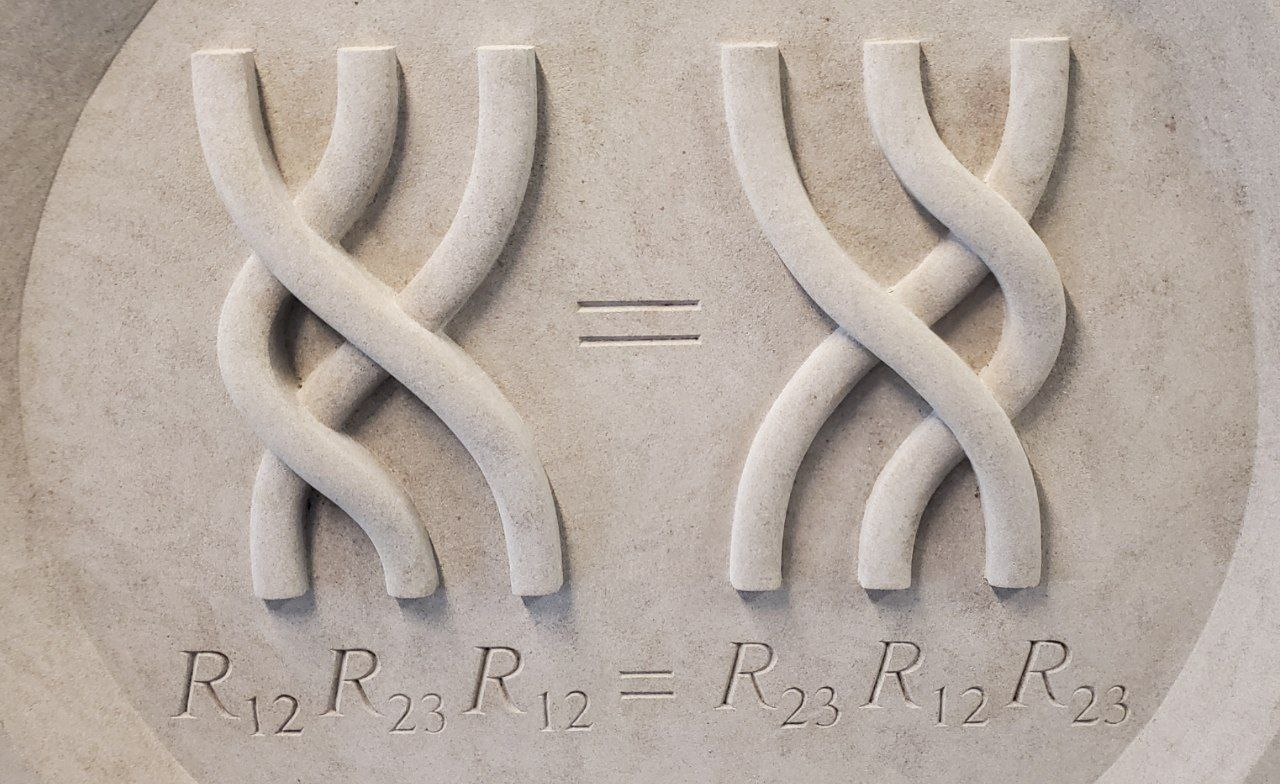
\includegraphics[width=0.4\textwidth]{ybe}
    \caption{Yang-Baxter equation sculpture at the Simons Center}
    \label{fig:ybe}
\end{figure}

Finally, we would like to reconstruct our quantum group given a family of $R$-matrices. We will do this using
\[ \text{Hopf algebra} \hookrightarrow \bigotimes V_{k_i}(a_i). \]
We can always assume that the collection of $V_i$ are closed under the tensor product. If we consider a physical space $V_i(a)$ and auxillary space $V_0(u)$, then matrix elements in $V_0$ give operators depending on $u$ in $V_i(a)$. These operators will generate $\mc{U}_{\hslash}$ and are closed under product (two auxillary spaces, one physical) and coproduct (one auxillary, two physical). Morphisms in the category of modules are maps commuting with $R$-matrices, and so we obtain relations in $\mc{U}_{\hslash}$. The $R$-matrix indeed gives braiding and commutation relations by the Yang-Baxter equations.

Now we will consider a family of subalgebras, called \textit{Baxter subalgebras}. Let $g \in \End(V_i(a_i))$ be such that $[g \otimes g, R] = 0$. These come from the Cartan torus, which in geometric cases come from discrete invariants. Then we consider the \textit{transfer matrix}
\[ \tr_1 (g \otimes 1) R_{V_i, V_j}(u/a). \]
These commute for fixed $g$ and all $V_i, u$, and so we get a family of commutative subalgebras in $\mf{U}_{\hslash}(\wh{g})$ which are parameterized by a maximal torus in $\mf{g}$.

More generally, we can have several strands on a cylinder and one strand going around as in~\Cref{fig:cylbraid} with the same condition on $g$ as before. But then we have commutativity with $g(a_i) = q a_i$, and so we get a canonical flat $q$-difference connection on $V_1(a_1) \otimes \cdots \otimes V_n(a_n)$, which is the qKZ equation.

\begin{figure}[h]
    \centering
    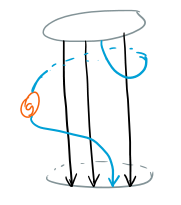
\includegraphics[width=0.3\textwidth]{cylbraid}
    \caption{Cylindrical braiding condition.}
    \label{fig:cylbraid}
\end{figure}

\subsection{Some more curve counting}

We now want to return to curve counting on fibrations
\[ A_r \hookrightarrow X \to B, \]
where for now we will specialize $B = \P^1$.

We will begin with Gromov-Witten theory. For example, when $r = 0$, then $X$ is the total space of two line bundles on $\P^1$, so above $0, \infty$ there are curves collapsed to a point and above the base there are copies of $\P^1$ mapping with degrees $\mu_i$. Therefore we have something like
\[ \sum_{\mu} \mr{edge}(\mu)^{-1} \times (\text{triple Hodge integral at $0$}) \times (\text{triple Hodge integral at $\infty$}). \]
The triple Hodge integral terms (\Cref{fig:thodge}) also involve nonsingular boundary conditions of tangency to $\pi^{-1}(\infty)$ (resp. $\pi^{-1}(0)$). Recall that we can break a curve in half while adding relative boundary conditions, and if we have $\P^1$ with a $\C^{\times}$ action, it can be broken in half with nonsingular boundary conditions into $\mr{edge}^{-1}$.

\begin{figure}[h]
    \centering
    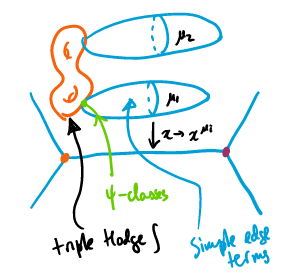
\includegraphics[width=0.4\textwidth]{triplehodge}
    \caption{Triple Hodge integral terms.}
    \label{fig:thodge}
\end{figure}

On the other side, in DT theory, a half edge corresponds to a 3D partition with extra boxes. 

The correspondences also include Givental's $J$-function for $\Hilb(\C^2, n)$, which is of course a Nakajima quiver variety.

Of course, whenever the target is a GIT quotient (for example in the case of a Nakajima variety), there is a notion of quasimaps~\cite{qmap}, which for $A_0$ are actually equal to Pandharipande-Thomas moduli spaces~\cite{pcmi}. For $r > 0$, these are not PT moduli spaces, but there is still a correspondence with PT-like theories~\cite{qmapsp}. The combinatorics of the PT vertex terms looks like~\Cref{fig:ptcomb}.

\begin{figure}[h]
    \centering
    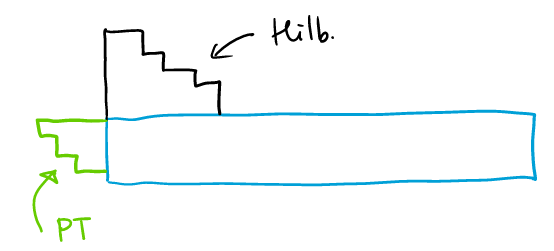
\includegraphics[width=0.4\textwidth]{ptcomb}
    \caption{Combinatorics of one-legged PT vertex.}
    \label{fig:ptcomb}
\end{figure}

The half-edge solves differential and difference equations (giving quantum groups) and are a much evolved relative of the hypergeometric function of the form
\[ \sum_{d \geq 0} z^d \prod_{i=1}^m \frac{(b_i)_d}{(a_i)_d} \]
where the $z$ are the K\"ahler variables (solving a linear differential equation) and the product term contains the equivariant variables (solving a linear difference equation).

\subsection{qKZ equation}

Donaldson-Thomas and quasimap theories make sense in $K$-theory, and so we obtain a $q$-difference equation from quantun groups, for example the qKZ equation. which comes from~\Cref{fig:cylbraid}. Here, the strands are $V_i(a_i)$ and we will call the blue strand $V_k(a_k)$. Recall that
\[ [g \otimes g, R] = 0, \]
and so we have 
\[ g = (\text{Loop rotation}) \cdot z, \]
where $z$ lives in the Cartan torus (also the K\"ahler variables) and the loop rotation is $T^{-1}$, where $Ta = qa$. 

Consider unrolling the cylinder into a hyperplane arrangement. Consider the simple example of hyperplanes $x_1=x2+\qty{-1,0,1}$ with walls like $x_1=x_3$ and $x_2=x_3$, see~\Cref{fig:hyperplane}. We can move in three directions, and in the first direction we obtain
\[ g^{(1)} R_{13} R_{12}. \]
In the second direction, we obtain
\[ g^{-(1)} R_{12}^{-1} g^{(1)} g^{(2)} R_{23} = g^{(2)} R_{12}^{-1} g^{-(2)} g^{(2)} R_{23}. \]

\begin{figure}[h]
    \centering
    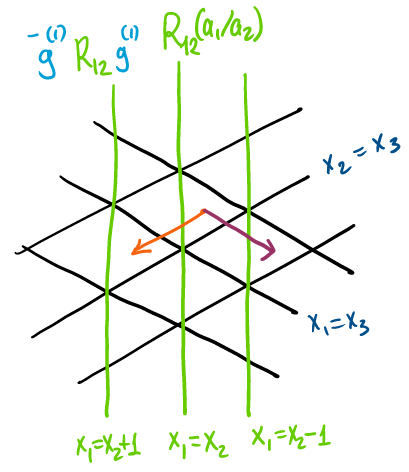
\includegraphics[width=0.4\textwidth]{hyperplane}
    \caption{Hyperplane arrangement}
    \label{fig:hyperplane}
\end{figure}

More generally, from each wall in our hyperplane arrangement $\ev{\alpha, x} + n = 0$, we obtain an operator $B_w(q^nx^{\alpha})$. If we consider $\lambda$ such that $\ev{\alpha, \lambda} \in \Z$ for all $\alpha$, then translation by $\lambda$ is conjugation by $\mc{O}(\lambda)$ of all $B_w$. This produces commuting $q$-difference operators, which are transition functions for a vector bundle of the form
\[ \C^{\mr{rank}} / q^{\mr{shifts}}. \]

For example, for $\mc{U}_{\hslash}(\wh{\mf{g}})$, we obtain the following:
\begin{enumerate}
    \item First, of course the qKZ equation, which depends on $z$ in the Cartan torus of $\mf{g}$.
    \item Universally, there exists a $q$-difference connection in $z$ that commutes with the qKZ operator. Operators in $\mc{U}_{\hslash}(\wh{\mf{g}})$ act on $V_1(a_1) \otimes \cdots \otimes V_n(a_n)$. This was studied first by Etingof-Varchenko~\cite{etvar} for finite-dimensional Lie algebras $\g$, where the $\alpha$ are simply the roots of $\mf{g}$. They write elements
        \[ B_w \in \mc{U}_{\hbar}(\mf{sl}_2) \hookrightarrow \mc{U}_{\hslash}(\wh{\g}), \]
        and these are called \textit{quantum dynamical Weyl groups}. More generally, Okounkov-Smirnov~\cite{qdenak} consider more complicated arrangements, for example for $\mc{U}_{\hslash}\qty(\wh{\wh{\mf{gl}(1)}})$, where we need all roots of of $\wh{\mf{gl}(1)}$, and so the hyperplane arrangement is $\Q$. This is clearly preserved by translation by $\Z$, so the root subalgebras are
        \[ \mc{U}_{\hslash}(\wh{\mf{gl}(1)}) \hookrightarrow \mc{U}_{\hslash}\qty(\wh{\wh{\mf{gl}(1)}}). \]
\end{enumerate}

The way to prove the above is to
\begin{enumerate}
    \item Find qKZ among the $q$-difference equations in the equivariant variables;
    \item Use commutation with qKZ and other known results to conclude.
\end{enumerate}

We know that $K(\Hilb(\C^2, \mr{pts}))$ is a module over a quantum group. Then
\[ K(\Hilb(\C^2, \mr{pts})) \otimes K(\Hilb(\C^2, \mr{pts})) = K(\mr{ideal} \oplus \mr{ideal}), \]
where $\mr{ideal} \oplus \mr{ideal}$ lives inside the space $M(2)$ of rank $2$ framed sheaves on $\C^2$. Here, a framed sheaf is a sheaf $\mc{F}$ on $\P^2$ such that 
\[ \mc{F}|_{\P^2 \setminus \C^2} \simeq \mc{O}_{\P^2\setminus \C^2}^{\oplus 2}. \]
Clearly, there is an action of $GL(2)$ on framed sheaves, so the sum of two ideals is the fixed locus of the maximal torus. Normalizing one of the weights of the torus, the locus of two ideals is the fixed locus of matrices of the form
\[ \mqty(a & 0 \\ 0 & 1), \]
and so shifts in $a$ give the qKZ equation.

\begin{rmk}
    The Hilbert scheme $\Hilb(\C^2, n)$ is the Nakajima quiver variety $M(n,1)$ for the quiver with one vertex and one loop.
\end{rmk}

Then the qKZ equation is
\[ (z \otimes 1)R_{12}(a) \]
and comes from a twist by $\mc{O}(1)$ in the framing. In the case of $A_r$ for $r > 0$, there are more fixed points of $a$ and there are ``constant sections'' whose degrees are encoded in the K\"ahler variables.

\subsection{Stable envelopes}

We would now like a map
\[ \on{Stab} \colon K(\Hilb) \otimes K(\Hilb) \to K(M(2)) \]
such that if we insert the relative conditions in the $A_r$-fibration, all contributions cancel except those of the constant curves. Once this \textit{stable envelope} exists, we will have
\[ R \approx \on{Stab}^T \cdot \on{Stab}. \]
Vanishing is easier in cohomology~\cite{qgqc}, but is more difficult in K-theory. The reason for this is that vanishing in $K$-theory is usually proved using rigidity (properness, which implies the result is a polynomial in $a$, and a degree bound, which implies the result has negative degree).

The stable envelope is supported on the full attracting locus inside $Y \times Y^a$ (or repelling for $\on{Unstab}$), which gives properness. For degree bounds, the Newton polygon
\[ \deg\qty(\on{Stab}|_{F_j \times F_i}) \]
is contained a fixed polygon.

\begin{rmk}
    Rigidity in K-theory should come from a rigidity argument in elliptic cohomology, where K-theory is thought of as coming from a nodal degeneration of an elliptic curve.
\end{rmk}

More abstractly, let $A$ be a torus acting on a variety $Y$. Then we choose a chamber in $\on{\ms{Lie}} A$, where the walls are weights on $N_{Y/Y^A}$. This is a choice of attracting and repelling directions and corresponds to $\xi \in \on{\ms{Lie}} A$ such that $Y^{\xi} \neq Y^A$. Now for all adjacent strata in our chamber structure, there should be an attaching map, and the attaching maps should commute. These can be constructed with some assumptions on $Y$, and now the $R$-matrix is simply the composition of one attaching operator and the inverse of the other. By the original commutation relation, we obtain the Yang-Baxter equation.

\begin{exm}
    If we consider the rank $r$ sheaves $M(r)$ and write $r = r_1 + r_2 + r_3$, then there is an action of $(\C^{\times})^3$. Therefore,
    \[ M(r)^A = M(r_1) \times M(r_2) \times M(r_3). \]
    More generally, for Nakajima varieties we can consider $w = \sum w^{(i)}$.
\end{exm}

\subsection{From enumerative geometry to quantum integrable systems}

A quantum integrable system is controlled by a commutative subalgebra of
\[ \End(H^*(\Hilb(A_r, \mr{pts}))). \]
One interesting problem is to find the eigenvectors and eigenvalues of this algebra. The Hilbert scheme of $A_r$ can be replaced by some Nakajima quiver variety
\[ \bigsqcup_v \mc{M}(v, w), \]
where the framing $w$ is fixed.

The quantum integrable system is actually the $q \to 1$ limit of some flat $q$-difference connection. In this setting, the problem of finding eigenthings is the problem of finding an integral solution to the $q$-difference connection. 

In the classical setting, consider a hyperplane arrangement and take hyperplanes
\[ \ev{\beta_1,x} = y_i = 0, \]
where the $\beta_1$ is fixed and the $y_i$ vary, then we obtain integrals that look like
\[ \int_{\gamma_j} \omega_i(x) \prod_m \qty(\ev{\beta_m, x} + y_m)^{c_m}, \]
where the $\omega_i(x)$ are rational and the $\gamma_j$ are homology classes on the complement of the hyperplane arrangement. This is like an Euler integral, which has the form
\[ \int x^{a-1}(x-1)^{b-1}(y-x)^{c-1} \dd{x}. \]
Our integral solves a differential equation (the Gauss-Manin connection) as well as a difference equation.

We now need to consider a $q$-analog. Here, the $\gamma_k$ will live on the complement of translates of subtori inside a tori, and the exponentials become gamma functions. Thus we are now integrating
\[ \int_{\gamma_j} \omega_i(x) \prod_m \frac{\Gamma_q(x^{m} a_m)}{\Gamma_q(x^{\beta_m}b_m)}, \]
which is a $q$-analog of a Mellin-Barnes integral. These are fundamental solutions $\Psi_{ij}$ to the $q$-difference equation.

The $q$-difference equation has the form 
\[ \Psi(qa) = M(a) \Psi(a). \]
In the $q \to 1$ limit, our solutions become
\[ e^{\frac{\int \log \lambda_j \frac{\dd{a}}{a}}{\log q}} \psi_j(a), \]
where $\psi_j(a)$ is the eigenvector with eigenvalue $\lambda_j(a)$. The eigenvectors and eigenvalues correspond to critical points of the $\int \log \lambda_j \frac{\dd{a}}{a}$ term, where the eigenvalues are $e^{\pdv{S}{a}}$ and the eigenvectors are given by evaluating $\omega_i(x)$ at the critical points $x$ of $S$. The $\omega_i(x)$ are called the \textit{off-shell Bethe eigenfunctions} and also depend on some auxillary variables. Note that we need to substitute in solutions of the \textit{Bethe equations} 
\[ \partial_x S = 0. \]

\begin{rmk}
    There is an important detail in which it is better to do the replacement
    \[ \int_{\gamma_j} \omega_i(x) \prod_m \frac{\Gamma_q(x^m a_m)}{\Gamma_q(x^{\beta_m} b_m)} \rightsquigarrow \int_{\norm{x}=1} \omega_i(x) \ell_j(x) \prod_m \frac{\Gamma_q(x^m a_m)}{\Gamma_q(x^{\beta_m} b_m)}. \]
\end{rmk}

Geometrically, we will work with quasimaps to Nakajima quiver varieties. The fundamental solution will correspond to the $\P^1$ with one nonsingular point and one relative point. On the other hand, the vertex (see~\cite[Section 7.4]{pcmi}) is the Mellin-Barnes integral.

\begin{exm}
    Consider $\mc{L} = \mc{O}(d)$ on $\P^1$. This has weight $w$ above $0$, $q$ along the $\P^1$, and $q^{-d} w$ above $\infty$. Therefore,
    \[ H^0(\mc{L}) = w + q^{-1} w + \cdots + q^{-d} w, \qquad H^1(\mc{L}) = 0 \]
    if $d > 0$, and so the Euler class is
    \[ \mr{Euler} = (1-w^{-1})(1-qw^{-1}) \cdots (1-q^dw^{-1}), \]
    which is a ratio of two $q$-gamma functions.
\end{exm}

The ideas in this example work more generally, and now it remains to find the elliptic term. This will come from some consideration of elliptic cohomology. The moduli space
\[ \ms{Qmap}(\P^1 \to \Hilb) \]
of quasimaps (or for a general Nakajima variety) has evaluation maps
\begin{equation*}
\begin{tikzcd}
    & \ms{Qmap}(\P^1 \to \Hilb) \ar{dl}{\mr{ev}_0} \ar{dr}{\mr{ev}_{\infty}} \\
    \text{ambient stack} & & \Hilb.
\end{tikzcd}
\end{equation*}
This gives us a push-pull morphism
\begin{equation*}
\begin{tikzcd}
    K(\text{ambient stack}) & & & K(\Hilb) \ar[swap]{lll}{\on{ev}_0(\wh{\mc{O}}^{\mr{vir}} \otimes \on{ev}_{\infty} \cdot z^{\deg})} \\
    \ms{Ell}() \ar{u}{\frac{\Gamma_q}{\Gamma_q}} & & & \ms{Ell}(\Hilb) \ar{u}{\frac{\Gamma_q}{\Gamma_q}} \ar{lll}{!}.
\end{tikzcd}
\end{equation*}
This gives us an elliptic function $\ell_j(x)$ which goes into the missing argument of the bottom-left $\ms{Ell}$. Also, the ratios of gamma functions were known to Iritani in the classical setting.

\begin{rmk}
    The consideration of elliptic cohomology does not affect the gamma function terms of the fundamental solution. The gamma function terms control the spectrum and can be observed already in the case of just one nonsingular point. This was observed already in~\cite{nekshat}.
\end{rmk}

\subsection{Elliptic cohomology}

Recall that
\[ H^*(\P^{n-1}, \C) = \C[x]/x^{n}, \]
where $x = c_1(\mc{O}(1))$. If we consider the action of $(\C^{\times})^n$, we can consider the \textbf{equivariant} cohomology 
\[ H_A^*(\P^{n-1}, \C) = H_A^*(\P^{n-1}, \C) = \frac{\C[x, a_1, \ldots, a_n]}{\prod_{i=1}^n (x+a_i)}. \]
This comes from the observation that $\P^n$ has $n$ ways to lift $x$ to an equivariant class (consider each of the toric divisors). If we consider
\[ \Spec H_A^*(\P^{n-1}, \C), \]
this is the union of hyperplanes $x = -a_i$, which are the cohomologies of the fixed points. Lifting to $k$-theory, we have the same picture after replacing $x=-a_i$ with $x=a_i^{-1}$ and taking $a \in A$ instead of $x \in \on{\ms{Lie}}(A)$.

Returning to the case of Nakajima varieties, the ring 
\[ K_{(\C^{\times})^2} (\Hilb(\C^2, n)) \]
is generated by the tautological bundle and its exterior powers. Then its spectrum
\[ \Spec K_{(\C^{\times})^2}(\Hilb(\C^2, n)) \]
is again a union of planes with data coming from plane partitions (which are the fixed points).

Finally, it makes sense to replace $\C^{\times}$ by $E = \C^{\times}/q^{\Z}$, where all of the exact same equations hold (subject to writing the group operation on $E$ as multiplication). The elliptic cohomology of $\Hilb(\C^2, n)$ is drawn in~\Cref{fig:ellhilbc2}.
\begin{figure}[h]
    \centering
    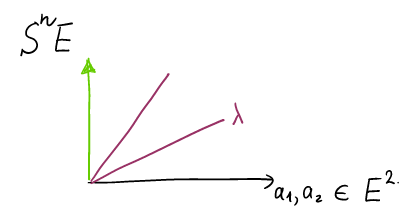
\includegraphics[width=0.4\textwidth]{ellhilbc2}
    \caption{Elliptic cohomology of $\Hilb(\C^2, n)$}
    \label{fig:ellhilbc2}
\end{figure}

\begin{rmk}
    It is important to note that $\ms{Ell}_G(X)$ is a \textbf{scheme} and not an algebra, so it is covariant in both $G$ and $X$.
\end{rmk}

Note that if $G$ is connected, then
\[ \ms{Ell}_G(\mr{pt}) = \ms{Ell}([\mr{pt}/G]) \]
is the moduli space of semistable degree $0$ $G$-bundles on the dual elliptic curve $E^{\vee}$. Also note that $\ms{Ell}_{(\C^{\times})^n}(\mr{pt}) = E^n$.

\subsection{Computations in elliptic cohomology of $\Hilb(\C^2, n)$}

In order to compute things, we need Euler classes. Suppose $p$ is a fixed point of $A$ acting on $X$, $V$ is a vector bundles, and $A$ acts with weights $w_i$ on $V_p$. Then
\[ \mr{Euler}(V)|_p = \begin{cases}
    \prod w_i & \text{in cohomology} \\
    \prod (1-w_i^{-1}) & \text{in K-theory} \\
    \prod \vartheta(w_i) & \text{in elliptic cohomology}.
\end{cases}
\]
Note that these theta functions are \textbf{not} functions but are sections of line bundles on elliptic curves. Recall that $V$ is a pullback
\begin{equation*}
\begin{tikzcd}
    V \ar{r} \ar{d} & \C^n/\mr{GL}(n) \ar{d} \\
    X \ar{r} & [\mr{pt}/\mr{GL}(n)].
\end{tikzcd}
\end{equation*}
This gives us a map
\[ \ms{Ell}(X) \to \ms{Ell}([\mr{pt}/\mr{GL}(n)]) = S^n E, \]
and on $S^n E$ there is the theta divisor $\Theta$, which is the locus of bundles with a section. Pulling back to $\ms{Ell}(X)$, we obtain a line bundle $\Theta(V)$, which is where $\mr{Euler}(V)$ lives.

Pushforwards in the elliptc theory involve Euler classes and thus twists by line bundles. If we use localization, we obtain the factors in~\Cref{tab:loccohkell}.
\begin{table}[H]
    \centering
    \caption{Localization in different cohomology theories}
    \label{tab:loccohkell}
    \begin{tabular}{ccc}
        \toprule
        In $H^*$ & In $K^*$ & In $\ms{Ell}$ \\
        \midrule
        $\frac{1}{\prod w_i}$ & $\frac{1}{\prod(1-w_i^{-1})}$ & $\frac{1}{\vartheta(w_i)}$ \\
        \bottomrule
    \end{tabular}
\end{table}
Then the pushforward $X \to \mr{pt}$ gives us a map $\Theta(TX) \to \ms{Ell}(\mr{pt})$ and the inclusion of a fixed point in $X$ gives us a map $\ms{Ell}(\mr{pt}) \to \Theta(TX)$.

\begin{rmk}
    There is an inclusion
    \[ \Pic(X) \otimes E \hookrightarrow \Pic_0(\ms{Ell}(X)). \]
    The K\"ahler variables live on the left hand side, and quantum computations in K-theory embed inside classsical computations in elliptic cohomology.
\end{rmk}

\begin{rmk}
    In principle, one could study enumerative counts in elliptic cohomology or even in another complex oriented cohomology theory like complex cobordism (see~\cite{cobpt}). However, we cannot form generating functions in these situations (for example in elliptic cohomology everything lives on a different line bundle), so we want to study the difference equations directly without generating functions.
\end{rmk}

We want to actually compute with the line bundles $\Theta(V)$ for vector bundles on $\Hilb(\C^2, n)$. For the tautological bundle, we have
\[ \deg \Theta(\mr{Taut}) |_{\lambda} = \sum_{\square} S^2\binom{1-j}{1-i} = \sum_{\square} \mqty{(j-1)^2 & (i-1)(j-1) \\ (i-1)(j-1) & (i-1)^2} \in S^2 \Z^2 = \mr{NS}(E^2). \]
For the tangent bundle, we obtain
\[ \deg \Theta(\mr{Tan})|_{\lambda} = \sum_{\square} S^2 \binom{a+1}{-\ell} + S^2 \qty\binom{-a}{\ell+1}. \]
Note that if we restrict $t_1t_2 = 1$, we have a square root. Thus, we can find a \textit{polarization}
\[ \mr{Tan} = T^{\frac{1}{2}} + t_1 t_2 (T^{\frac{1}{2}})^{\vee}. \]
Thus we will need sections of a line bundle of the form
\[ \mc{L} = \sqrt{\Theta(\mr{Tan})} \otimes \Pic_0(\ms{Ell}). \]
We will call the determinant $\det \mr{Taut} \eqqcolon \mc{O}(1)$. Recall that taking the determinant corresponds to taking
\[ (x_1, \ldots, x_n) \in S^n E \to E \ni \prod x_i. \]
Now recall that $\Pic_0(E) = E^{\vee} = E$, so for $z \in \Pic_0(E)$ (the K\"ahler variable), we can consider the meromorphic section
\[ \frac{\vartheta\qty(\prod x_i z)}{\vartheta\qty(\prod x_i) \vartheta(z)} \]
of some degree $0$ line bundle. More generally, we can take $z \in \Pic(X) \otimes E$.

Recall that we have a map
\[ \ms{Ell}(\Hilb) \to \ms{Ell}(\text{ambient stack}). \]
We want to take a Lagrangian class on $\Hilb$ and extend it to the ambient stack. This is like taking a section of a line bundle $\mc{S}$ on $\ms{Ell}(\Hilb)$ and extending it to the ambient stack. The ambient stack has a Harder-Narasimhan stratification in which the stable locus is the first piece. This allows us to take an inductive approach to the interpolation, see~\cite{indconststab}. There is a nonabelian analogue of this, see~\cite{nonabstab}.

One step of the induction is the following. Consider the inclusion $U = X \setminus \mr{Attr}(F) \hookrightarrow X$. Then in ordinary cohomology, we have the long exact sequence
\[ \cdots \to H^i(X, U) \to H^i(X) \to H^i(U) \to \cdots \]
By Atiyah-Bott, the normal bundle $N_{X/\mr{Attr}(F)}$ has a nontrivial action, so all of the connecting maps vanish. By excision, we can replace $(X, U)$ by an embedding of $F$ into a vector bundle $V$ over $F$, which produces
\[0 \to H^i(\mr{Thom}(V)) \to H^i(V) \to H^i(V \setminus 0) \to 0. \]
In elliptic cohomology, we obtain an exact sequence of line bundles. Consider the diagram
\begin{equation*}
\begin{tikzcd}
    V \ar{d} \ar{r} & { [\C^n/\mr{GL}(r)] } \ar{d}  & { [(\C^n \setminus 0) / \mr{Gl}(r)] } \ar[l, phantom, "\supset"] \ar[equal]{r} & { [\mr{pt}/\mr{Gl}(r-1)] } \\
    F \ar{r} & { [\mr{pt}/\mr{GL}(r)] }.
\end{tikzcd}
\end{equation*}
This produces us an inclusion $\ms{Ell}(V \setminus 0) \hookrightarrow \ms{Ell}(V)$, which gives us the divisor $\Theta(V)$ on $\ms{Ell}(V)$. From a section of $\mc{L} |_{\Theta(V)}$, we have an exact sequence
\[ 0 \to \mc{S} \otimes \Theta(-V) \to \mc{S} \to \mc{S}|_{\Theta(V)} \to 0. \]
In studying sheaves on $\ms{Ell}(F)$, we want global sections. Consider the long exact cohomology sequence
\[ 0 \to H^0(\mc{S} \otimes \Theta(-V)) \to H^0(\mc{S}) \to H^0(\mc{S}|_{\Theta(V)}) \to H^1(\mc{S} \otimes \Theta(-V)) \to \cdots. \]
Note that because $\mc{S} \in \Theta(T^{\frac{1}{2}}) \otimes \Pic_0$, $\mc{L} \coloneqq \mc{S} \otimes \Theta(-V)$ has degree $0$. It is also nontrivial (sections have poles related to enumerative geometry). However, if $\mc{S}$ is a nontrivial degree $0$ line bundle on an abelian variety $\mc{E}$, it has no cohomology whatsoever.

We have now produced a stable envelope
\[ \mr{Stab} \colon \ms{Ell}(\text{stable}) \to \ms{Ell}(\mr{stack}) \]
which interpolates sections of line bundles. We also have the traditional elliptic stable envelope~\cite{ellstab}
\[ \on{Stab} \colon \ms{Ell}(X^A) \to \ms{Ell}(X). \]
As we change attracting and repelling directions, we obtain elliptic $R$-matrices. The K-theoretic and cohomological versions can be obtained using degeneration.

\subsection{Quantum q-difference equations}

We would like to solve these equations using integrals. Recall that in K-theory, we have
\begin{equation*}
\begin{tikzcd}
    K(\mr{stable}) \ar{rrr}{\on{ev}_0 (\on{ev}_{\infty}^{-1} \otimes \wh{\mc{O}}^{\mr{vir}} z^{\deg})} & & & K(\mr{stack})[[z]] \\
    K(\mr{stable}) \ar{u}{(\mr{Iritani})\Gamma_q} \ar{rrr}{\ch(\on{Stab}_{\ms{Ell}})} & & & K(\mr{stack})(z) \ar{u}.
\end{tikzcd}
\end{equation*}
Recall that the solutions are of the form
\[ \Psi_{ij} = \int_{\abs{x}=1} \omega_i(x) \ell_j(x) \prod \frac{\Gamma_q}{\Gamma_q}. \]
As $q \to 1$, the gamma functions give the Bethe equation, while the $\omega_i(x)$ are the $q=0$ limit of the $\ell_i(x)$ in~\cite{qmapbethe}. This is called the \textit{off-shell Bethe eigenfunction}. For quotients by groups of the form $\prod GL(V_i)$, the nonabelian stable envelope reduces to the abelian one, so there is a formula in terms of $R$-matrices.

Consider the $XXZ$ spin chain, where we have states like $\uparrow \downarrow \downarrow \uparrow \downarrow \downarrow \downarrow$. Take the vacuum to be $\downarrow \cdots \downarrow$. Then the physical diagram will look like~\Cref{fig:xxzspin}.
\begin{figure}[h]
\begin{center}
\begin{tikzpicture}[scale=0.9, transform shape]
    \draw[-] (-4,2) -- (-4,-2);
    \draw[-] (-3,2) -- (-3,-2);
    \draw[-] (-2,2) -- (-2,-2);
    \draw[-] (-1,2) -- (-1,-2);
    \draw[-] (0,2) -- (0,-2);
    \draw[-] (1,2) -- (1,-2);
    \draw[-] (2,2) -- (2,-2);
    \draw[-] (3,2) -- (3,-2);
    \draw[-] (4,2) -- (4,-2);
    \draw[-] (-5,1) -- (5,1);
    \draw[-] (-5,0) -- (5,0);
    \draw[-] (-5,-1) -- (5,-1);
    \node[text=blue] at (-4,2.3) {$\boldsymbol{\downarrow}$};
    \node[text=blue] at (-3,2.3) {$\boldsymbol{\downarrow}$};
    \node[text=blue] at (-2,2.3) {$\boldsymbol{\downarrow}$};
    \node[text=blue] at (-1,2.3) {$\boldsymbol{\downarrow}$};
    \node[text=blue] at (0,2.3) {$\boldsymbol{\downarrow}$};
    \node[text=blue] at (1,2.3) {$\boldsymbol{\downarrow}$};
    \node[text=blue] at (2,2.3) {$\boldsymbol{\downarrow}$};
    \node[text=blue] at (3,2.3) {$\boldsymbol{\downarrow}$};
    \node[text=blue] at (4,2.3) {$\boldsymbol{\downarrow}$};
    \node[text=blue] at (-4,-2.3) {$\boldsymbol{\downarrow}$};
    \node[text=green] at (-3,-2.3) {$\boldsymbol{\uparrow}$};
    \node[text=blue] at (-2,-2.3) {$\boldsymbol{\downarrow}$};
    \node[text=blue] at (-1,-2.3) {$\boldsymbol{\downarrow}$};
    \node[text=green] at (0,-2.3) {$\boldsymbol{\uparrow}$};
    \node[text=green] at (1,-2.3) {$\boldsymbol{\uparrow}$};
    \node[text=blue] at (2,-2.3) {$\boldsymbol{\downarrow}$};
    \node[text=blue] at (3,-2.3) {$\boldsymbol{\downarrow}$};
    \node[text=blue] at (4,-2.3) {$\boldsymbol{\downarrow}$};
    \node[text=blue] at (-5.2,1) {$\boldsymbol{\downarrow}$};
    \node[text=blue] at (-5.2,0) {$\boldsymbol{\downarrow}$};
    \node[text=blue] at (-5.2,-1) {$\boldsymbol{\downarrow}$};
    \node[text=green] at (5.6,1) {$\boldsymbol{\uparrow}(u_1)$};
    \node[text=green] at (5.6,0) {$\boldsymbol{\uparrow}(u_2)$};
    \node[text=green] at (5.6,-1) {$\boldsymbol{\uparrow}(u_3)$};
    \node at (0,2.8) {$T^* \mr{Gr}(0,9)$};
    \node at (-6.3,0) {$T^* \mr{Gr}(0,3)$};
    \node at (7.1,0) {$T^* \mr{Gr}(3,3)$};
    \node at (0,-2.8) {$T^* \mr{Gr}(3,9)$};
\end{tikzpicture}
\end{center}
\caption{Example of XXZ spin chain}%
\label{fig:xxzspin}
\end{figure}
If the spectral variables $u_i$ solve the Bethe equation, then the bottom state is an eigenvector. This is the origin of the algebraic Bethe ansatz.

In our setting, consider the picture of~\Cref{fig:statmechnak}.
\begin{figure}[h]
\begin{center}
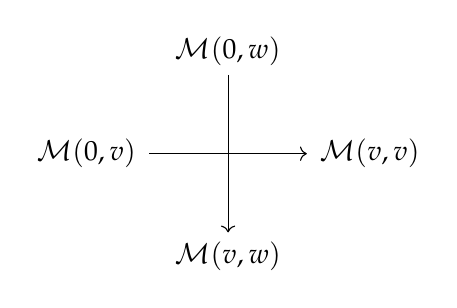
\begin{tikzpicture}[scale=1, transform shape]
    \draw[->] (-1,0) -- (1,0);
    \draw[->] (0,1) -- (0,-1);
    \node at (-1.8,0) {$\mc{M}(0, v)$};
    \node at (1.8,0) {$\mc{M}(v, v)$};
    \node at (0,1.3) {$\mc{M}(0, w)$};
    \node at (0,-1.3) {$\mc{M}(v, w)$};
\end{tikzpicture}
\end{center}
\caption{Simple model for Nakajima varieties}%
\label{fig:statmechnak}
\end{figure}
The analog of all up arrows here is when $v = w$ and the maps $W \to V$ are isomorphisms while the maps $V \to W$ are zero. This happens because the Bethe roots sit inside a maximal torus of $\prod GL(W_i) = \prod GL(V_i)$ here.

\subsection{An open problem}

In dimension $1$, we computed the equivariant $\P^1$ in terms of the action of $GL(\infty)$ on the Fock space and concluded that the $\P^1$ with two marked points is a $\tau$-function for the 2-Toda hierarchy. This comes from the action of $GL(\infty)$ on $\mr{Fock} \otimes \mr{Fock}$, which has the action of $\sum \psi_i \otimes \psi_i^*$

In dimension $3$, we know both the equivariant $\P^1$ with one marked and one nonsingular point and with one marked point and one relative point in terms of $\mc{U}_{\hslash} \qty(\wh{\wh{\mf{gl}(1)}})$. In the $\hslash=1$ limit, we recover $\mc{U}(\mf{gl}(\infty))$, which corresponds to going down to $1$ dimension. If we take $\mc{U}_{\hslash}$ acting on $\mr{Fock} \otimes \mr{Fock}(\mr{shift})$ along with a screening operator, where
\[ \mr{Fock} = \bigoplus_{n \geq 0} K(\Hilb(\C^2, n)), \]
what is the deformation of 2-Toda? 

The case of one marked point and one relative point is rational in $z$~\cite{ratcapdescvertex}. Three key facts are
\begin{enumerate}
    \item The equivariant $\P^1$ with one descendent and one relative condition vanishes for $\mc{M}(v, w)$ for $w \gg 0$ (the so-called large framing vanishing)~\cite{pcmi}.
    \item Splitting the equivariant $\P^1$ in half and adding two nonsingular points, consider $w = w_0 + w_1$, where $w_0$ is fixed and $w_1$ is large. Then $a \in \C^{\times}$ acts on $W_1$ by scaling. We now have
        \[ \mc{M}(\cdot, w)^a = \mc{M}(\cdot, w_0) \times \mc{M}(\cdot, w_1), \]
        so the descendent is a Laurent polynomial in the Chern roots of the tautological bundle $V$. Twisting by $\det V$, we obtain an ordinary polynomial. Localizing on $\P^1$ and $a$ and taking $a \to 0$, we reduce to computing the same descendent for $w = w_0$.
    \item In the $a \to 0$ limit, the fundamental solution for the $q$-difference equation becomes the product of an explicit fusion operator and two fundamental solutions.
\end{enumerate}

\chapter{Double ramification cycles and integrable hierarches (Paolo Rossi and Alexandr Buryak)}%

\textbf{Note:} see~\cite{rossisurvey} for a complete discussion.

\section{Integrable systems}

\subsection{Notation and formalism}

We will precisely define things like the KdV equation, tau functions, and higher symmetries. This comes from a formal algebraic discussion of things like dynamical systems. For a detailed reference, see~\cite{dubzhang}. Define the \textit{phase space}
\[ \mc{P} \coloneqq \qty{u \colon S^1 \to \C^n} \]
We consider the coordinates $u^{\alpha} \colon S^1 \to \C$ as formal variables. Also, we will let $x$ be the coordinate on $S^1$.

\begin{defn}
    A \textit{differential polynomial} is an element of the ring
    \[ \wh{\mc{A}} \coloneqq \C[[u^*]][u_{>0}^*][[\ep]], \]
    where $u_k^{\alpha} = \partial_x^k u^{\alpha}$. This has a grading where $u_k^*$ has degree $k$ and $\ep$ has degree $-1$.
\end{defn}

This is not quite a ring of functions on $\mc{P}$, so we will correct this. Define the operator
\[ \partial_x \colon \wh{\mc{A}} \to \wh{\mc{A}} \qquad \partial_x = \sum_{k \geq 0} u_{k+1}^{\alpha} \pdv{u_k^{\alpha}}. \]
This gives us a space $\wh{\mc{F}} = \wh{\mc{A}}/(\Im \partial_x \oplus \C)$ of \textit{local functionals} and should be thought of as integrating over the $S^1$. There is a way to reintroduce a ring structure on local functionals, but it will not be necessary for our purposes.

As changes of coordinates on the phase space, consider the \textit{Miura transformations}
\[ \wt{u}^{\alpha} = \wt{u}^{\alpha}(u_*^*, \ep) \in \in \wh{\mc{A}}^{[0]}. \]
For some amount of invertibility, we require
\[ \deg \qty(\pdv{\wt{u}^{\alpha}}{u^{\beta}}) \neq 0, \qquad u_*^* = 0, \qquad \ep = 0. \]

\begin{rmk}
    Miura transformations are invertible in the sense that they can be solved for $u^*$ as a system of ODEs order by order in $\ep$.
\end{rmk}

We may define \textit{Fourier coordinates} on $\mc{P}$ by taking the substitution
\[ u^{\alpha} \sum_{b \in \Z} p_b^{\alpha} (e^{ix})^b. \]
Here, the $p_b^{\alpha}$ are the Fourier coordinates. We force the coefficients to have polynomial dependence on $b$ and to sum to $0$ in analogy with the Fourier transform.

\subsection{Poisson structure}

We will now place a Poisson structure
\[ \qty{-,-} \colon \wh{\mc{F}} \times \wh{\mc{F}} \to \wh{\mc{F}} \]
on $\mc{P}$ or equivalently on $\wh{\mc{F}}$. Here, we take
\[ \qty(\int f \dd{x}, \int g \dd{x}) \mapsto \int \fdv{\ol{f}}{u^{\alpha}} K^{\alpha\beta} \qty(\fdv{\ol{g}}{u^{\beta}}) \dd{x}, \]
where $\ol{f} = \int f \dd{x}$ and the \textit{variational derivatives} are defined by
\[ \pdv{\ol{f}}{u^{\alpha}} = \sum_{k \geq 0} (-\partial_x)^k \pdv{f}{u_k^{\alpha}} \colon \wh{\mc{F}} \to \wh{\mc{A}} \] 
and the Poisson operator $K^{\alpha\beta}$ is defined by
\[ K^{\alpha\beta} = \sum_{j \geq 0} K_j^{\alpha\beta} \partial_x^j \qquad K_j^{\alpha\beta} \in \wh{\mc{A}}^{[-j+1]}. \] 
This is not quite a Poisson structure in general as we still need to impose skew-symmetry and the Jacobi identity.

\subsection{System of evolutionary PDEs}

A \textit{system of evolutionary PDEs} (or a vector field on $\mc{P}$) is a differential equation
\[ \pdv{u^{\alpha}}{t} = Q^{\alpha(u_*^*, \ep)} \in \wh{\mc{A}}^{[1]}, \]
where $Q^{\alpha}$ is a differential polynomial. Analogously, recall that a vector field $X$ on a finite-dimensional manifold can be written as either
\[ X = X^{\alpha} \pdv{x^{\alpha}} \]
or as 
\[ \dv{x^{\alpha}}{t} = X^{\alpha}(x^1, \ldots, x^n). \]

Define the operator
\[ L_{\nu}^{\beta} = \sum_{s \geq 0} (-\partial_x)^s \circ \pdv{\wt{u}^{\beta}}{u_s^{\nu}} \]
and its adjoint
\[ (L^*)_{\mu}^{\alpha} = \sum_{s \geq 0} \pdv{\wt{u}^{\alpha}}{u_s^{\mu}} \partial_x^s. \]
This is related to coordinate transformations on tensors by the formula
\[ K_{\wt{u}}^{\alpha\beta} = (K^*)_{\mu}^{\alpha} \circ K^{\mu\nu} \circ L_{\nu}^{\beta}. \]

\begin{thm}[\cite{darbouxhamiltonian}]
    There exists a Miura transformation bringing any Poisson structure of the form
    \[ K^{\alpha\beta} = g^{\alpha\beta}(u^*) \partial_x + b_{\gamma}^{\alpha\beta}(u^*) u_1^{\gamma} + O(\ep) \]
    with $g^{\alpha\beta}$ a nondegenerate flat metric on $\C^n$ to the form
    \[ K_{\wt{u}}^{\alpha\beta} = \eta^{\alpha\beta} \partial_x \]
    where $\eta^{\alpha\beta}$ nondegenerate constant symmetric. Note that the Jacobi identity imposes that the $b_{\gamma}^{\alpha\beta}$ are the Christoffel symbols for the Levi-Cevita connection of $g^{\alpha\beta}$, see~\cite{dubnov}.
\end{thm}

\begin{exm}[KdV equation]\label{exm:kdv}
    Let $\mc{P} = \qty{u \colon S^1 \to \C}$. Then the ring of differential polynomials is
    \[ \wh{\mc{A}} = \C[[u]] [u_{>0}] [[\ep]] \]
    and we will consider the vector field
    \[ \pdv{u}{t} = u u_1 + \frac{\ep^2}{12} u_3. \]
    This is a Hamiltonian operator for the Poisson structure, where $K = \partial_x$. The Hamiltonian that produces this system is
    \[ \ol{h} = \int \qty(\frac{u^3}{6} + \frac{\ep^2}{12} u u_2) \dd{x} \in \wh{\mc{F}}^{[0]}. \]
    Now we can compute
    \begin{align*}
        \pdv{u}{t} &= K \qty(\pdv{\ol{h}}{t}) \\
        &= \partial_x \qty(\frac{u^2}{2} + \frac{\ep^2}{24} u_2 + \partial_x^2 \qty(\frac{\ep^2}{2u}u)) \\
        &= \partial_x \qty(\frac{u^2}{2} + \frac{\ep^2}{12} u_2),
    \end{align*}
    which is exactly the differential polynomial we want.
\end{exm}

We now want to lift $K^{\alpha\beta}$ to a map
\[ \wh{\mc{A}} \times \wh{\mc{F}} \to \wh{\mc{A}}. \]
There is a standard way to do such a thing by taking
\[ \qty{f, \ol{g}} = \sum_{k \geq 0} \pdv{f}{u_k^{\alpha}} \partial_x^k \qty(K^{\alpha\beta} \qty(\fdv{\ol{g}}{u^{\beta}})). \]
In \Cref{exm:kdv}, we computed the vector field $K \qty(\pdv{\ol{h}}{u}) = \qty{u, \ol{h}}$.

\begin{exm}[2-KdV equation]
    Consider $\mc{P} = \qty{u \colon S^1 \to \C^2}$ and the Hamiltonian
    \[ \ol{h} = \int \frac{(u^1)^2}{2} u^2 + \frac{(u^2)^4}{36} + \qty(-\frac{1}{2} (u_1^1)^2 - \frac{1}{24} u^2 (u_1^2)^2)\ep^2 + \frac{1}{432} (u_2^2)^2 \ep^4 \dd{x}. \]
    Also, consider the Poisson operator
    \[ K = \mqty(0 & 1 \\ 1 & 0) \partial_x. \]
    The resulting PDE is called the 2-KdV equation.
\end{exm}

\subsection{Integrable systems and tau-structures}

Consider a collection of Hamiltonians
\[ \qty{\ol{h}_{\alpha, d}}_{\substack{\alpha = 1, \ldots, N \\ d \geq 0}} \]
that commute with respect to the Poisson structure, i.e.
\[ \qty{\ol{h}_{\alpha_1, d_1}, \ol{h}_{\alpha_2, d_2}} = 0 \]
for all $\alpha_1, \alpha_2 = 1, \ldots, N$ and $d_1, d_2 \geq 0$. We obtain the differential equation
\[ \pdv{u^{\alpha}}{t_{d_1}^{\alpha_1}}{t_{d_2}^{\alpha_2}} = \pdv{u^{\alpha}}{t_{d_2}^{\alpha_2}}{t_{d_1}^{\alpha_1}}, \]
or symmetry of the mixed partials. Then our differential equations can be written as
\[ \pdv{u^{\alpha}}{t_d^{\beta}} = \qty{u^{\alpha}, \ol{h}_{\beta, d}}, \qquad \Vectorstack{{\alpha, \beta = 1, \ldots, N} {d \geq 0}}. \]
Commutativity guarantees the existence of a formal solution
\[ u^{\alpha}(x, t_*^*, \ep) \in \C[[x, t_*^*, \ep]] \]
with the initial condition
\[ u^{\alpha}(x, t_*^* = 0, \ep) = \ol{u}(x, \ep). \]

We will now discuss $\tau$-structures. Assume that 
\[ \partial_{t_0^1} u^{\alpha} = K^{\alpha\mu} \fdv{\ol{h}_{1,0}}{u^{\mu}} = u_x^{\alpha}. \]
Then a \textit{$\tau$-structure} is a choice of $h_{\beta, d} \in \wh{\mc{A}}^{[0]}$ for $\beta = 1, \ldots, N$ and $d \geq -1$ such that
\begin{enumerate}
    \item $K^{\alpha\mu} \fdv{\ol{h}_{\beta,-1}}{u^{\mu}} = 0$ for all $\beta, \alpha = 1, \ldots, N$;
    \item The integrals of the $h_{\beta, d}$ satisfy
        \[ \int h_{\beta, d} \dd{x} = \ol{h}_{\beta, d}. \]
    \item There is an equality of Poisson brackets
        \[ \qty{h_{\beta_1, d_1-1}, \ol{h}_{\beta_2, d_2}} = \qty{h_{\beta_2, d_2-1}, \ol{h}_{\beta_1, d_1}} \]
        for all $\beta_1, \beta_2 d_1, d_2$.
\end{enumerate}

Assuming that a tau-structure exists, we see that
\[ \qty{h_{\beta_1, d_1-1}, \ol{h}_{\beta_2, d_2}} = \partial_x \Omega_{\beta_1, d_1; \beta_2, d_2} \in \wh{\mc{A}}^{[0]}. \]
The third condition implies that
\[ \Omega_{\beta_1, d_1; \beta_2, d_2} = \Omega_{\beta_2, d_2; \beta_1, d_1}. \]

\begin{rmk}
    For all solutions
    \[ u^{\alpha}(x, t_*^*, \ep) \in \C[[x, t_*^*, \ep]] \]
    of the integrable system, there exists a unique $F \in \C[[t_*^*, \ep]]$ such that
    \[ \Omega_{\beta_1, d_1; \beta_2, d_2} |_{u^*=u^*(x, t_*^*, \ep)} |_{x=0} = \pdv{F(t_*^*, \ep)}{t_{d_1}^{\beta_1}}{t_{d_2}^{\beta_2}}. \]
\end{rmk}

For example, the definition of the tau-structure tells us that
\begin{align*} 
    \partial_x \Omega_{\beta_1, d_1; 1, 0} &= \pdv{h_{\beta_1, d_1-1}}{t_0^1} \\
    &= \partial_x h_{\beta_1, d_1-1}.
\end{align*}
In particular, we obtain
\[ \Omega_{\beta_1, d_1; 1, 0} = h_{\beta_1, d_1-1}. \]

Assume that $K_u^{\alpha\beta}|_{\ep = 0} = \eta^{\alpha\beta} \partial_x$. Then
\[ h_{\beta, -1} |_{\ep = 0} = \eta_{\beta \mu} u^{\mu}, \]
so in particular
\[ h_{\beta, -1} = \eta_{\beta \mu} u^{\mu} + O(\ep). \]

\begin{defn}
    Given a tau-structure, its system of \textit{normal coordinates} is
    \[ \wt{u}^{\alpha} = \eta^{\alpha \mu} h_{\mu, -1}(u_*^*, \ep) = u^{\alpha} + O(\ep). \]
    Note that
    \[ \eta_{\alpha\mu} \wt{u}^{\mu} |_{u^*=u^*(x,t_*^*,\ep)} |_{x=0} = \pdv{F}{t_0^1}{t_0^{\alpha}}. \]
\end{defn}

\subsection{KdV hierarchy revisited}

Recall the Hamiltonian
\[ \ol{h} = \int \qty(\frac{u^3}{6} + \frac{\ep^2}{24} uu_2) \dd{x}, \]
and consider $K = \partial_x$. Then we see that
\[ u_t = u u_x + \frac{\ep^2}{12} u_{x x x}. \]
We will now give a new construction of the KdV hierarchy.

\begin{thm}[\cite{recdrhierarchy}]
    Define $g_d \in \wh{\mc{A}}^{[0]}$ for $d \geq -1$ via $g_{-1} = u$ and
    \[ \partial_x (D-1) g_{d+1} = \qty{g_d, \ol{h}}, \]
    where we choose
    \[ D = \ep \pdv{\ep} + \sum_{k \geq 0} u_k \pdv{u_k}. \]
    Then
    \[ \qty{\ol{g}_{d_1}, \ol{g}_{d_2}} = 0. \]
    Note that
    \[ \ol{g}_0 = \int \frac{u^2}{2} \dd{x}. \]
\end{thm}

\begin{lem}
    Let $K^{\alpha\beta} = \eta^{\alpha\beta} \partial_x$ be in the full Getzler normal form and
    \[ \ol{g}_{\alpha,d} = \pdv{g_{\alpha,d+1}}{u^1}. \]
    Then 
    \[ h_d \coloneqq \fdv{\ol{g}_{d+1}}{u} \]
    is a tau-structure.
\end{lem}

\begin{proof}
    We will suppress the Greek indices. We now compute
    \begin{align*}
        0 &= \pdv{u} \qty{\ol{g}_{d_1}, \ol{g}_{d_2}} \\
        &= \qty{\pdv{\ol{g_{d_1}}}{u}, \ol{g}_{d_2}} + \qty{\ol{g}_{d_1}, \pdv{\ol{g}_{d_2}}{u}} \\
        &= \qty{h_{d_1-1}, \ol{h}_{d_2}} + \qty{\ol{h}_{d_1}, h_{d_2-1}}.
    \end{align*}
    By antisymmetry, we obtain a tau-structure.
\end{proof}

Using this tau-structure, we can write the following well-known result:
\begin{thm}[\cite{wittenconj}]
    The $\tau$-function $F(t_*, \ep)$ for the solution of the KdV hierarchy with initial condition
    \[ u(x, t_* = 0, \ep) = X \]
    is
    \[ F(t_*, \ep) = \sum \frac{\ep^{2g}}{n!} \int{\ol{\mc{M}}_{g, n}} \psi_1^{d_1} \cdots \psi_n^{d_n} t_{d_1} \cdots t_{d_n}. \]
\end{thm}

We would like to consider changes of coordinates that preserve tau-structures. These are called \textit{normal Miura transformations}. Let 
\[ \qty{h_{\alpha,d}, \qty{-,-}}_{\substack{\alpha = 1,\ldots,N \\ d \geq -1}} \]
be an integrable system with tau-structure. Recall that we have normal coordinates
\[ \wt{\mu}^{\alpha} = \eta^{\alpha \mu} h_{\mu,-1}. \]
Fix a differential polynomial $P \in \wh{\mc{A}}^{[-2]}$. The \textit{normal Miura transformation} generated by $P$ is
\begin{align*}
    \wt{\wt{u}}^{\alpha} &= \wt{u}^{\alpha} + \eta^{\alpha \mu} \partial_x \qty{P, \ol{h}_{\mu, 0}} \\
    &= \wt{\mu}^{\alpha} + \eta^{\alpha \mu} \pdv{P}{x}{t_0^{\mu}}.
\end{align*}
Then
\begin{align*}
    h'_{\alpha,d} &= h_{\alpha,d} + \partial_x \qty{P, \ol{h}_{\alpha,d+1}} \\
    &= h_{\alpha,d} + \pdv{P}{x}{t_{d+1}^{\alpha}}
\end{align*}
is a tau-structure for
\[ \qty{h'_{\alpha, d} |_{\wt{\mu}(\wt{\wt{u}}_*^*, \ep)}, K_{\wt{\wt{u}}}}. \]

\begin{rmk}
    Note that for all solutions, the tau-function changes under normal Miura transformations as
    \[ \wt{F}(t_*^*, \ep) = F(T_*^*, \ep) + P|_{\wt{u} = \wt{u}(x, t_*^*, \ep)}|_{x=0}. \]
\end{rmk}


\section{Double ramification hierarchy}

Recall that if $K^{\alpha\beta} = \eta^{\alpha\beta} \partial_x + O(\ep)$, then
\begin{align*}
    \qty{\ol{h}_{\alpha_1, d_1}, \ol{h}_{\alpha_2, d_2}} &= \int \fdv{\ol{h}_{\alpha_1, d_1}}{u^{\mu}} (\eta^{\mu \nu} \partial_x + O(\ep)) \fdv{\ol{h}_{\alpha_2, d_2}}{u^{\nu}} \dd{x} \\
    &= \int \qty(\pdv{h_{\alpha_1, d_1}^{[0]}}{u^{\mu}} \eta^{\mu\nu} \pdv{h_{\alpha_2, d_2}^{[0]}}{u^{\nu}} + O(\ep)) \dd{x}.
\end{align*}
Because the integrand is now a total derivative in $x$, commutativity of the Hamiltonians (in the dispersionless limit) requires that
\[ \pdv{h^{[0]}_{\alpha_1, d_1}}{u^{\beta}}{u^{\mu}} \eta^{\mu \nu} \pdv{h_{\alpha_2, d_2}^{[0]}}{u^{\nu}}{u^{\gamma}} \]
is invariant under exchanging $\beta, \gamma$. This encodes relations on $\ol{\mc{M}}_{0, 4}$, where points $2, 3$ have insertions $\psi^{d_1}, \psi^{d_2}$, which should be invariant under exchange of $1, 4$. Therefore, we should think of commutativity under exchange of indices as the WDVV equation. However, this approach only works in genus $0$.

We will now define
\[ \ol{h}_d^{[0]} = \sum_{n \geq 2} \frac{1}{n!} \qty(\int_{\ol{\mc{M}}_{0,1+n}} \psi_1^d) u^n \]
and for any cohomological field theory,
\[ \ol{h}_{\alpha, d}^{[0]} = \sum_{n \geq 2} \frac{1}{n!} \qty(\int_{\ol{\mc{M}}_{0, 1+n}}C_{0, 1+n}\qty(e_{\alpha} \otimes \bigotimes_{i=1}^n e_{\alpha_i})) u^{\alpha_1} \cdots u^{\alpha_n}. \]

\subsection{Double ramification cycle}

Define the \textit{double ramification cycle} $\mr{DR}_g(a_1, \ldots, a_n) \in \mc{R}^g \subset H^{2g}(\ol{\mc{M}}_{g, n}, \C)$ as follows. First, define
\[ \ol{\mc{M}}_{g, n}^{\sim}(\P^1, A) = \qty{\Sigma \to (\P^1, 0, \infty)} / \C^{\times}. \]
This has a morphism
\[ p \colon \ol{\mc{M}}_{g, n}^{\sim}(\P^1, A) \to \ol{\mc{M}}_{g, n}, \]
and so we may define
\[ \mr{DR}_g(A) \coloneqq p_* [\ol{\mc{M}}_{g, n}^{\sim}(\P^1, A)]^{\mr{vir}}. \]
This is a tautological cycle, and $\mr{DR}_g(A) = 0$ unless $\sum a_i = 0$. Recently, an explicit formula was found by Janda-Pandharipande-Pixton-Zvonkine~\cite{drcycles}.

Now define a compact type version
\begin{align*} 
    \mr{DR}_g^{\mr{ct}}(A) &= \frac{1}{g!} \Theta^g \\
    &= \frac{1}{g!} \qty(-\frac{1}{4} \sum_{J \subset \qty{1, \ldots, n}} \sum_{h=0}^g a_J^2 \delta_h^J)^g,
\end{align*}
where $a_J = \sum_{i \in J} a_i$ and $\delta_h^J$ is the cycle corresponding to the stable graph with genus $h$ with $J$ marked points and genus $g-h$ with $J^c$ marked points. Note $\delta_0^{\qty{i}} = - \psi_i$. Also note that
\[ \lambda_g \mr{DR}_g(A) = \lambda_g \mr{DR}_g^{\mr{ct}}(A). \]

Instead of working with $\ol{\mc{M}_{0, n}}$, we need to work with the Losev-Manin compactification
\[ \mc{LM}_{0, \abs{\text{ramification}}} \]
of the moduli space of curves. Now we have a diagram
\begin{equation*}
\begin{tikzcd}
    & \ol{\mc{M}}_{g, n}^{\sim}(\P^1, A) \ar{dl}{b_{\gamma}} \ar{dr}{p} \\
    \mc{LM}_{0,-} & & \ol{\mc{M}}_{g, n}.
\end{tikzcd}
\end{equation*}
The Losev-Manin compactifications still have the WDVV equation, so we have the formula
\begin{align*}
    0 &= p_* b_{\gamma}^* (\mr{WDVV}) \\
    &= \sum_{\substack{I \sqcup J = \qty{1, \ldots,n} \\ g_1+g_2+r-1=g}} \mr{DR}_{g_1}(0_x, A_I, \kappa_1, \ldots, \kappa_r) \boxtimes \mr{DR}_{g_2}(0_y, A_J, -\kappa_1, \ldots, -\kappa_r)\frac{\kappa_1 \cdots \kappa_r}{r!}.
\end{align*}
Here, $x, y$ are internal marked points on the two components, and our expression must be invariant under exchanging $x, y$.

\subsection{Formation of integrable hierarchy}

We are now ready to define
\[ \ol{g}_{\alpha, d} = \sum \frac{(-\ep^2)^g}{n!} \qty(\int_{\ol{\mc{M}}_{g, n}} \mr{DR}_g(0, a_1, \ldots, a_n) \psi^d C_{g, n}\qty(e_{\alpha} \otimes \bigotimes_{i=1}^n e_{\alpha_i})) \prod_{i=1}^n p_{a_i}^{\alpha_i} \]
for any cohomological field theory. We now attach the Poisson structure
\[ \qty{p_a^{\alpha}, p_b^{\beta}} = a \delta_{a+b} \eta^{\alpha\beta}. \]
We can see that
\[ \qty{\ol{g}_{\alpha, d}, \ol{g}_{\beta, d}} = k \pdv{\ol{g}_{\alpha, d}}{p_k^{\mu}} \eta^{\mu\nu} \pdv{\ol{g}_{\beta,d}}{p_{-k}^{\nu}} \]
It is unclear that this vanishes, and in fact we will need to quantize our integrable hierarchy or correct our formulas. 

To make corrections in the classical case, we will add $\lambda$-classes to the WDVV equation as follows:
\[ \sum_{\substack{I \sqcup J = \qty{1, \ldots,n} \\ g_1+g_2+r-1=g}} \lambda_{g_1} \mr{DR}_{g_1}(0_x, A_I, \kappa_1, \ldots, \kappa_r) \boxtimes \lambda_{g_2} \mr{DR}_{g_2}(0_y, A_J, -\kappa_1, \ldots, -\kappa_r)\frac{\kappa_1 \cdots \kappa_r}{r!}. \]
Then our Hamiltonians become
\[ \ol{g}_{\alpha, d} = \sum \frac{(-\ep^2)^g}{n!} \qty(\int_{\ol{\mc{M}}_{g, n}} \lambda_g \mr{DR}_g(0, a_1, \ldots, a_n) \psi^d C_{g, n}\qty(e_{\alpha} \otimes \bigotimes_{i=1}^n e_{\alpha_i})) \prod_{i=1}^n p_{a_i}^{\alpha_i}. \]

Our system is related to the formalism of the previous section by taking the Fourier expansion
\[ u^{\alpha} = \sum_{a \in \Z} p_a^{\alpha} e^{iax}. \]
Now our Poisson bracket takes the form
\[ K^{\alpha\beta} = \eta^{\alpha\beta} \partial_x. \]
We may now rewrite our Hamiltonians as differential polynomials by
\[ \ol{g}_{\alpha, d} \sum \frac{\ep^{2g}}{n!} \qty[a_1^{k_1} \cdots a_n^{k_n}] \qty(\int_{\ol{\mc{M}}_{g, n}} \lambda_g \mr{DR}_g(0, a_1, \ldots, a_n) \psi^d C_{g, n}\qty(e_{\alpha} \otimes \bigotimes_{i=1}^n e_{\alpha_i})) u_{k_1}^{\alpha_1} \cdots u_{k_n}^{\alpha_n}. \]
Note here that $\lambda_g \mr{DR}_g(a_1, \ldots, a_n) \in \mc{R}^g[a_1, \ldots, a_n]^{2g}$.

\begin{lem}
    If $C_{g, n}$ is a cohomological field theory with unit $e_1$, then
    \[ \pdv{\ol{g}_{d+1}}{u^1} = \ol{g}_d. \]
\end{lem}

\begin{cor}
    The DR hierarchy is $\tau$-symmetric with
    \[ h_{\alpha, d} = \fdv{\ol{g}_{\alpha,d+1}}{u^1}. \]
\end{cor}

This leads naturally to the following conjecture:
\begin{conj}[\cite{taudrhierarchy}]\label{conj:drdz}
    The DR hierarchy is normal Miura equivalent to the Dubrovin-Zhang hierarchy.
\end{conj}

\subsection{Quantization}

Define
\[ \ol{G}_{\alpha, d} = \sum \frac{\hslash^g}{n!} \qty(\int_{\ol{\mc{M}}_{g, n}} \Lambda \qty(\frac{-\ep^2}{\hslash}) \mr{DR}_g(0, A) \psi_1^d C_{g,n+1}(e_{\alpha} \otimes e_B))p_A^B. \]
The Poisson bracket is defined by
\[ \qty[p_a^{\alpha}, p_b^{\beta}] = \eta^{\alpha\beta} a \delta_{a+b,0} \hslash. \]
To compute the commutator of two local functionals, we need to take a deformation of the Moyal product for the old Poisson structure as follows:
\[ \ol{f} \star \ol{g} = \ol{f} \qty(e^{\sum_{k \in \Z} \hslash^2 k \overset{\shortleftarrow}{\partial}_{p_{-k}} \vec{\partial}_{p_k}}) \ol{g} \]
and then take
\[ [\ol{f}, \ol{g}] = \ol{f} \star \ol{g} - \ol{g} \star \ol{f}. \]

\begin{thm}
    The Hamiltonians $\ol{G}_{\alpha, d}$ commute:
    \[ \qty[\ol{G}_{\alpha_1, d_1}, \ol{G}_{\alpha_2, d_2}] = 0. \]
\end{thm}

\subsection{DR hierarchy for DR cycles}

Recall that the double ramification cycles satisfy the following properties:
\begin{itemize}
    \item $\mr{DR}_0(a_1, \ldots, a_n) = 1 \in H^0(\ol{\mc{M}}_{g, n})$. Therefore, $\mr{DR}_0(a, b, 0) = \delta_{a+b,0} \in H^0(\ol{\mc{M}}_{0,3})$;
    \item $\mr{DR}_g(0, \ldots, 0) = (-1)^g \lambda_g$;
    \item If $\pi \colon \ol{\mc{M}}_{g, n+1} \to \ol{\mc{M}}_{g, n}$ is the forgetful map, then
        \[ \mr{DR}_{g}(a_1, \ldots, a_n, 0) = \pi^* \mr{DR}_g(a_1, \ldots, a_n); \]
    \item If $\on{gl} \colon \ol{\mc{M}}_{g_1, n_1+1} \times \ol{ \mc{M}}_{g_2, n_2+1}  \to \ol{\mc{M}}_{g,n}$ is the gluing map, then
        \[ \on{gl}^* \mr{DR}_g(a_1, \ldots, a_n) = \mr{DR}_{g_1}\qty(a_{i_1}, \ldots, a_{i_{n_1}}, -\sum a_{i_k}) \otimes \mr{DR}_{g_2}\qty(a_{j_1} \ldots, a_{j_{n_2}}, -\sum a_{j_k}). \]
\end{itemize}

We would now like to compute the flows corresponding to this partial CohFT. Here, set
\begin{align*} 
    \ol{g}_{0,1} &= \sum_{g, n} \frac{(-\ep^2)^g}{n!} \sum_{\alpha_i, a_i} \qty[\int_{\ol{\mc{M}}_{g, n+1}} \psi_1 \lambda_g C_{g, n+1}\qty(e_0 \otimes \bigotimes_{i=1}^n e_{\alpha_i}) \mr{DR}_g(0, a_1, \ldots, a_n)] p_{a_1}^{\alpha_1} \cdots p_{a_n}^{\alpha_n} \\
    &= \sum_{g, n} \frac{(-\ep^2)^g}{n!}(2g-2+n) \int_{\ol{\mc{M}}_{g, n}} \lambda_g C_{g, n}\qty(\bigotimes_{i=1}^n e_{\alpha_i}) \mr{DR}_g(a_1, \ldots, a_n) p_{a_1}^{\alpha_1} \cdots p_{a_n}^{\alpha_n}.
\end{align*}
Substituting our double ramification cycles for the $C_{g, n}$ terms, this integral vanishes unless $n=3$.

\begin{thm}[\cite{drnckdv}]
    There is the explicit formula
    \[ \int_{\ol{\mc{M}}_{g, 3}} \lambda_g \mr{DR}_g(a_1, a_2, a_3) \mr{DR}_g(b_1,b_2, b_3) = \frac{(a_1b_2 - a_2 b_1)^{2g}}{2^{3g}g!(2g+1)!!} \]
    for all $g \geq 0$.
\end{thm}

\begin{proof}
    We will begin with Hain's formula
    \[ \mr{DR}_g(a_1, \ldots, a_n) |_{\mc{M}_{g, n}^{\mr{ct}}} = \frac{1}{g!} \Theta(a_1, \ldots, a_n)^g|_{\mc{M}_{g, n}^{\mr{ct}}}, \]
    where
    \[ \Theta(a_1, \ldots, a_n) = \sum_{j=1}^n \frac{a_j^2 \psi_j}{2} - \frac{1}{4} \sum_{h=0}^g \sum_{J \subset [h]} a_J^2 \delta_h^J. \]
    Moreover, we have
    \[ \Theta(a_1, \ldots, a_n)^{g+1} |_{\mc{M}_{g, n}^{\mr{ct}}} = 0. \]
    Then the Hodge classes vanish outside of the compact type locus, so we now need to prove that
    \[ f_{g}(\ol{a}, \ol{b}) \coloneqq \int_{\ol{\mc{M}}_{g,3}} \lambda_g \Theta(\ol{a})^g \mr{DR}_g(\ol{b}) =\frac{(a_1b_2 - a_2 b_1)^{2g}}{2^{3g}g!(2g+1)!!}. \]
    Our main tool is an explicit formula for $a_s \psi_s \mr{DR}_g(a_1, \ldots, a_n)$ analogous to our formula for the WDVV equation:
    \begin{align*} 
        a_s \psi_s \mr{DR}_g(a_1, \ldots, a_n) ={} & \sum_{\substack{I \sqcup J = [n] \\ a_I > 0}} \sum_{p \geq 1} \sum_{g_1+g_2+p-1 = g} \sum_{k_1,\ldots,k_p \geq 1} \frac{\rho}{2g-2+n} \frac{\prod_{i=1}^p k_i}{p!} \times \\
        & \times \mr{DR}_{g_1}(A_I, -k_1, \ldots, -k_p) \boxtimes \mr{DR}_{g_2}(A_J, k_1, \ldots, k_p),
    \end{align*}
    where
    \[ \rho = \begin{cases}
        2g_2-2+\abs{J}+p & s \in I \\
        2g_1 - 2 + \abs{I} + p & s \in J.
    \end{cases}
    \]
    If we add Hodge classes, this formula simplifies to become
    \[ \lambda_g a_s \psi_s \mr{DR}_g(a_1, \ldots, a_n) = \sum_{\substack{I \sqcup J = [n] \\ s \in I}} \sum_{g_1+g_2 = g} \frac{2g_2-1+\abs{J}}{2g-2+n} a_I \lambda_{g_1} \mr{DR}_{g_1}(A_I, -a_I) \boxtimes \lambda_{g_2}\mr{DR}_{g_2}(A_J, a_I). \]
    We are now ready to compute
    \begin{align*} 
        \int_{\ol{\mc{M}}_{g,3}} \Theta(\ol{a})^{g-1} &\lambda_g \psi_i \mr{DR}_g(\ol{b}) =  \\
        ={}& \frac{2g-1}{2g+1} \sum_{g_1+g_2=g} \int_{\ol{\mc{M}}_{g,3}} \lambda_g \Theta(\ol{a})^{g-1} \mr{DR}_{g_1}(b_i,-b_i) \boxtimes \mr{DR}_{g_2}(b_j,b_k, b_i) \\
        & -\frac{2}{2g+1} \sum_{g_1+g_2 = g} \frac{b_j}{b_i} \int_{\ol{\mc{M}}_{g,3}} \lambda_g \Theta(\ol{a})^{g-1} \mr{DR}_{g_1}(b_i,b_j,b_j) \boxtimes \mr{DR}_{g_2}(b_j,-b_j) \\
        & -\frac{2}{2g+1} \sum_{g_1 + g_2 = g} \frac{b_k}{b_i}\int_{\ol{\mc{M}}_{g,3}} \lambda_g \Theta(\ol{a})^{g-1} \mr{DR}_{g_1}(b_i, b_j, b_j) \boxtimes \mr{DR}_{g_2}(b_k,-b_k).
    \end{align*}
    The first term becomes
    \[ \sum_{\substack{h_1+h_2 = g-1 \\ g_1+g_2 =  g}} \binom{g-1}{h_1} \int \qty(\Theta(a_i,-a_i)^{h_1} \lambda_{g_1} \mr{DR}_{g_1}(b_i,-b_i)) \boxtimes (\Theta(a_j, a_j, a_i)^{h_2} \lambda_{g_2} \mr{DR}_{g_2}(b_j, b_k, b_i)). \]
    The integral splits as
    \[ \qty[\int_{\ol{\mc{M}}_{g_1, 2}} \Theta(a_i,-a_i)^{h_i} \lambda_{g_1} \mr{DR}_{g_1}(b_i,-b_i)]\qty[\int_{\ol{\mc{M}}_{g_2,3}} \Theta(a_j, a_k, a_i)^{h_2} \lambda_{g_2} \mr{DR}_{g_2}(b_j, b_k, b_i)]. \] 
    The first integral in this product vanishes unless $h_1=g_1-1, h_1 = 0$, in which case it is is
    \[ a_i^{2h_1} \Theta(1,-1)^{h_1} \lambda_{g_1} b_i^{2g_1} \Theta(1, 01)^{g_1}, \]
    and therefore the overall integral becomes
    \[ \qty[\int_{\ol{\mc{M}}_{1,2}}\lambda_1 \mr{DR}(b_i, -b_i)] \qty[\int_{\ol{\mc{M}}_{g-1,3}}\Theta(a_j, a_k, a_i)^{g-1} \lambda_{g-1}\mr{DR}_{g-1}(b_j, b_k, b_i)] = \frac{b_i^2}{24} f_{g-1}(\ol{a}, \ol{b}). \]
    We can use the same ideas for the other terms, and we obtain
    \[ \int_{\ol{\mc{M}}_{g, 3}} \Theta(\ol{a})^{g-1}\lambda_g \psi_i \mr{DR}_g(\ol{b}) = \frac{(2g+1)b_i^2 - 6 b_jb_k}{24(2g+1)}f_{g-1}(\ol{a}, \ol{b}). \]
    We can use the same ideas to compute
    \[ \int_{\ol{\mc{M}}_{g,3}}\lambda_g \Theta(\ol{a})^{g-1} \delta_h^J \mr{DR}_g(\ol{b}). \]
    Finishing the computation, we obtain
    \[ f_g(a, b) = \frac{(a_1b_2 - a_2 b_1)^2}{8(2g+1)} f_{g-1}(a,b). \qedhere \]
\end{proof}

For any $a \in \Z$, we now obtain
\begin{align*}
    \pdv{u^a}{t_1^0} &= \partial_x \sum_{g \geq 0} \frac{\ep^{2g}}{2} \sum_{a_1+a_2=a} \sum_{d_1+d_2 = 2g} [b_1^{d_1} b_2^{d_2}] \qty(\int_{\ol{\mc{M}}_{g,n}} \psi_1 \lambda_g) \\
    &= \partial_x \sum_{g \geq 0} \frac{\ep^{2g}}{2} \sum \sum [b_1^{d_1} b_2^{d_2}] \qty[\frac{(a_1b_2 - a_2 b_1)^{2g}}{2^{3g}g! (2g-1)!!} u_{d_1}^{a_1} u_{d_2}^{a_2}] \\
    &= \partial_x \sum_{g \geq 0} \frac{\ep^{2g}}{2} \sum \sum [b_1^{d_1} b_2^{d_2}] \qty[\frac{(a_1b_2 - a_2 b_1)^{2g}}{2^{2g}(2g)!!}] u_{d_1}^{a_1} u_{d_2}^{a_2} \\
    &= \partial_x \sum_{g \geq 0} \frac{\ep^{2g}}{2 \cdot 2^{2g}} [b_1^{d_1} b_2^{d_2}] \qty[\sum h_1+h_2=2g \frac{1}{h_1! h_2!}(a_1b_2)^{h_1}(-a_2b_1)^{h_2}] u_{d_1}^{a_1} u_{d_2}^{a_2} \\
    &= \partial_x \sum_{g \geq 0} \frac{\ep^{2g}}{2 \cdot 2^{2g}} \sum h_1+h_2=2g \frac{1}{h_1! h_2!} a_1^{h_1}(-a_2)^{h_2} (\partial_x^{h_2}u^{a_1})(\partial_x^{h_1} u^{a_2}).
\end{align*}
Using the Fourier expansion, we now obtain
\begin{align*}
    \pdv{u^a}{t_1^0} &= \frac{1}{2} \partial_x \sum_{g \geq 0} \frac{\ep^{2g}}{2^{2g}} \sum_{h_1+h_2=2g} \frac{1}{h_1!}{h_2!} a_1^{h_1}(-a_2)^{h_2} (\partial_x^{h_2}u^{a_1}) e^{ia_1y} (\partial_x^{h_1} u^{a_2}) e^{ia_2 y}  \\
    &= \frac{1}{2} \partial_x \sum_{g \geq 0} \frac{1}{2^{2g}} \sum_{h_1+h_2=2g} \frac{(i\ep)^{2g}}{h_1! h_2!}(-1)^{h_2} (\partial_x^{h_2} \partial_y^{h_1} u)(\partial_x^{h_1} \partial_y^{h_2}u).  \\
\end{align*}
Here, we see the Moyal star-product
\[ f \star_{\hslash} g = f \exp\qty(\frac{i\hslash}{2} (\overset{\shortleftarrow}{\partial}_x \vec{\partial}_y - \overset{\shortleftarrow}{\partial_y} \vec{\partial}_x))g, \]
and therefore we obtain
\[ \pdv{u}{t_1^0} = \frac{1}{2} \partial_x (u \star_{\ep} u). \]
More generally, we have
\[ \pdv{u}{t_d^0} = \frac{1}{(d+1)!} \partial_x \qty(\underbrace{u \star_{\ep} \cdots \star_{\ep} u}_{d+1\text{ times}}). \]

\subsection{Noncommutative integrable hierarchy}

We now want to consider
\[ C_{g,n}\qty(\bigotimes e_{a_i}) = \exp(\mu^2 \Theta(a_1, \ldots, a_n)). \]
Then the flows $\pdv{t_d^0}$ of the DR hierarchy begin with
\[ \pdv{u}{t_1^0} = \frac{1}{2} \partial_x(u \star_{\ep\mu} u) + \frac{\ep^2}{12} u_{x x x}, \]
which is a kind of noncommutative KdV equation. The higher flows are the higher flows of the ncKdV hierarchy, which can be described using the Lax representation. This leads naturally to the next problem:

\begin{prob}
    How can we describe the flows $\pdv{t_d^{\alpha}}$ with $\alpha \neq 0$?
\end{prob}

There are of course other questions, including the relationship with the Dubrovin-Zhang hierarchy as in~\Cref{conj:drdz}, which implies the following conjecture.
\begin{conj}[\cite{nckdvpixton}]
    Intersection numbers with Pixton's class give a solution of the noncommutative KdV hierarchy.
\end{conj}

\chapter{Airy ideals and topological recursion: an investigative tool for enumerative geometry, VOAs, and gauge theories (Vincent Bouchard)}%

Topological recursion was invented by Eynard-Orantin in their work~\cite{toprecursion} on matrix models in 2007 and then reformulated in terms of Airy structures (or Airy ideals) by Kontsevich-Soibelman~\cite{airytoprec} in 2017. This is a correspondence between geometry, algebra, and differential equations.

\section{Witten's conjecture}

This story began with theories of 2d quantum gravity.
Define the \textit{partition function}
\[ \mc{Z} = \exp \qty(\sum_{\substack{g=0 \\ n=1 \\ 2g-2+n>0}}^{\infty} \frac{\hslash^{2g-2+n}}{n!} \sum_{k_1, \ldots, k_n} F_{g,n}[k_1, \ldots, k_n] t_{k_1} \cdots t_{k_n}), \]
where we define
\[ F_{g,n}[k_1, \ldots, k_n] = \int_{\ol{\mc{M}}_{g,n}} \psi_1^{k_1} \cdots \psi_n^{k_n}. \]
To simplify our notation, we will write
\[ \mc{Z} = \exp \qty(\sum_{k=1}^{\infty} \hslash^k q^{(k+2)}(t_A)). \]

\begin{thm}[\cite{wittenconj}]\label{thm:witten}
    The function
    \[ u(t_0, t_1, \ldots) = \pdv[2]{t_0} \log \mc{Z} \]
    is the unique solution to the KdV hierarchy with initial condition $u(t_0, 0, \ldots) = t_0$.
\end{thm}

\subsection{Reformulation as differential constraints for $\mc{Z}$}

For $k \geq -1$, define the operator
\[ L_k = J_{k+1} - \frac{1}{2} \sum_{m+n=k-1} :J_m J_n: - \delta_{k,0} \frac{\hslash^2}{8}, \]
where
\[ J_m = \hslash \pdv{t_m}, m \geq 0 \qquad J_{-m} = \hslash(2m-1)t_{m-1}, m \geq 1. \]
Now we can reformulate~\Cref{thm:witten} as
\begin{thm*}
    $\mc{Z}$ is the unique solution to the constraints $L_k \mc{Z} = 0$ for all $k \geq -1$.
\end{thm*}

Note that the $L_k$ satisfy the relation
\[ [L_i, L_j] = \hslash^2(i-j)L_{i+j}. \]
Thus we have a representation of a subalgebra of the Virasoro algebra, which is defined by
\[ [L_i, L_j] = \hslash^2(i-j)L_{i+j} \frac{\hslash^4 c}{12} i^2(i-1) \delta_{i, -j} \]
Note that $L_k$ has the expansion
\[ L_k = \hslash \pdv{t_{k+1}} + O(\hslash^2), \]
which makes it easy to see uniqueness once we have existence.

\subsection{Potential generalizations}

The first possible generalization is the Virasoro conjecture~\cite{virasoroconj}, where we remove uniqueness of the solution and preserve the geometry (using Gromov-Witten theory of projective varieties) and the Virasoro algebra. This has been proved in several cases, including toric varieties~\cites{virasorofanotoric}{virasorotoric}, flag varieties~\cite{virasoroflag}, Grassmannians~\cite{virasorograss}, varieties with semisimple quantum cohomology~\cite{2dsscohft}, Calabi-Yau varieties~\cite{virasorogw}, and toric bundles over varieties satisfying the Virasoro conjecture~\cite{virasorotoricbundle}. There is also progress on Virasoro constraints for sheaf-counting theories, see~\cite{virasoropt}.

The second possible generalization is to keep existence and uniqueness of the solution $\mc{Z}$ to the constraints $H_i \mc{Z} = 0$. More precisely, we want to find constraints on $H_i$ such that $H_i \mc{Z} = 0$ always has a unique solution of the form
\[ \mc{Z} = \exp \qty(\sum_{k=1}^{\infty} \hslash^k q^{(k+2)}(x_A)) \]
with the initial condition $\mc{Z} \_{x_A = 0} = 1$. This is the generalization that we will take.

\section{Airy ideals}

\subsection{Weyl algebra and modules}

Let $A$ be a (possibly infinite) indexing set. The \textit{Weyl algebra} $\mc{D}_A$ is defined as 
\[ \mc{D}_A = \C[x_A] \ev{\partial_A} / ([\partial_i, x_j] = \delta_{ij}). \]
This is only a filtered algebra, so it is difficult to form power series. We will use the \textit{Rees construction} to turn it into a graded algebra.

Here, we will use the filtration
\[ \qty{0} \subseteq F_0 \mc{D}_A \subseteq F_1 \mc{D}_A \subseteq \cdots \subseteq \mc{D}_A, \]
where
\[ F_i \mc{D}_A = \qty{\sum_{m+k\leq i} P_{a_1, \ldots, a_m}^{(k)}(x_A) \partial_{a_1} \cdots \partial_{a_m}}. \]
For example, $F_2 \mc{D}_A$ contains terms like $x_1$ and $x_1 \partial_2$ but not terms like $x_1^2 \partial_2$.

Now we may define the \textit{Rees Weyl algebra}
\[ \mc{D}_A^{\hslash} = \bigoplus_{k=0}^{\infty} \hslash^k F_k \mc{D}_A, \]
where $\deg \hslash = 1$, and the completion
\[ \wh{\mc{D}}_A^{\hslash} = \prod_{k=0}^{\infty} \hslash^k F_k \mc{D}_A. \]
This is in fact a good way to handle power series, and we will consider $H_i \in \wh{\mc{D}}_A^{\hslash}$.

We will now consider the polynomial module $\mc{M}_A$, which has the following properties: 
\begin{itemize}
    \item $\mc{M}_A$ is generated by $1 \in \mc{M}_A$; 
    \item The annihilator $\on{Ann}_{\mc{D}_A}(1)$ is the left ideal generated by $\partial_i$; 
    \item We recover 
        \[ \mc{D}_A / \on{Ann}_{\mc{D}_A}(1) \simeq \mc{M}_A. \]
\end{itemize}
We can now introduce $\hslash$ directly into our module, but we need a filtration on $\mc{M}$ such that
\[ F_i \mc{D} \cdot F_j \mc{M} \subset F_{i+j} \mc{M}. \]
A natural choice is to let $F_i \mc{M}_A$ be polynomials of degree at most $i$. We can now repeat the Rees construction by considering
\[ \mc{M}_A^{\hslash} = \bigoplus_{k=0}^{\infty} \hslash^k F_k \mc{M}_A, \qquad \wh{\mc{M}}_A^{\hslash} = \prod_{k=0}^{\infty} \hslash^k F_k \mc{M}_A. \]
The partition function $\mc{Z}$ will live in a twist of $\wh{\mc{M}}_A^{\hslash}$ rather than in the module itself. Some properties of $\hslash$ are as follows:
\begin{itemize}
    \item $\wh{\mc{M}}_A^{\hslash}$ is a cyclic left $\wh{\mc{D}}_A^{\hslash}$-module generated by $1$;
    \item $\on{Ann}_{\wh{\mc{D}}_A^{\hslash}}(1)$ is the left ideal $\mc{I}_{\mr{can}}$ generated by $\hslash \partial_i$;
    \item We can recover the module by
        \[ \wh{\mc{D}}_A^{\hslash}/\mc{I}_{\mr{can}} = \wh{\mc{M}}_A^{\hslash}. \]
\end{itemize}

We can now reformulate our problem as
\begin{prob}
    What conditions should a left ideal $\mc{I} \subset \wh{\mc{D}}_A^{\hslash}$ satisfy such that $\mc{I} \cdot \mc{Z}$ has a unique solution of the form
    \begin{equation}\label{eqn:desiredsoln}
        \mc{Z} = \exp\qty(\sum_{k=1}^{\infty} \hslash^k q^{(k+2)}(x_A))? 
    \end{equation}
\end{prob}

\subsection{Characterization of ideals solving our problem}

From our expression for $\mc{Z}$, it is clear that the operators
\[ \ol{H}_i = \hslash \partial_i - \sum_{k=1}^{\infty} \hslash^{k+1} \partial_i q^{(k+2)}(x_A) \]
satisfy $\ol{H}_i \mc{Z} = 0$. Denote the ideal generated by the $\ol{H}_i$ by $\ol{\mc{I}}$, which is in fact $\on{Ann}_{\wh{\mc{D}}_A^{\hslash}}(\mc{Z})$.

\begin{defn}
    Define an automorphism $\Phi \colon \wh{\mc{D}}_A^{\hslash} \to \wh{\mc{D}}_A^{\hslash}$ by
    \[ \Phi \colon (\hslash, \hslash x_i, \hslash \partial_i) \mapsto \qty(\hslash, \hslash x_i, \hslash \partial_i - \sum_{k=1}^{\infty} \hslash^{k+1} \partial_i q^{(k+2)}(x_A)). \]
    Note that this is a valid construction because $[\ol{H}_i, \hslash x_j] = \hslash^2 \delta_{ij}$ and $[\ol{H}_i, \ol{H}_j] = 0$.
\end{defn}

Given the twist $\Phi$, define the twisted module ${}^{\Phi}\wh{\mc{M}}_A^{\hslash}$ by the twisted product
\[ \wh{\mc{D}}_A^{\hslash} \cdot^{\Phi} \wh{\mc{M}}_A^{\hslash} \to \wh{\mc{M}}_A^{\hslash} \qquad P \cdot^{\Phi} f = \Phi^{-1}(P) \cdot f. \]
This satisfies the same properties as the untwisted version. Because $\Phi(P) = \mc{Z} \cdot P \cdot \mc{Z}^{-1}$, we can define a \textit{module of exponential type} by $\mc{Z} \wh{\mc{M}_A^{\hslash}}$, which is cyclic and generated by $\mc{Z}$. Clearly we have
\[ \on{Ann}_{\wh{\mc{D}}_A^{\hslash}}(\mc{Z}) = \Phi(\mc{I}_{\mr{can}}) = \ol{\mc{I}}. \]

\begin{defn}[Airy ideal]
    Let $\ol{\mc{I}} \subseteq \wh{\mc{D}}_A^{\hslash}$ be a left ideal. It is \textit{Airy} if it is generated by $(\ol{H}_i)_{i \in A}$.
\end{defn}

\begin{thm}
    The function $\mc{Z}$ defined in~\Cref{eqn:desiredsoln} is the unique solution to $\ol{\mc{I}} \cdot \mc{Z} = 0$ with $\mc{Z} |_{x_A = 0} = 1$.
\end{thm}

Of course, any ideal can have many different generating sets. How can we recognize Airy ideals in a more intrinsic manner?

\begin{thm}{\cite{airytoprec}}\label{thm:charairy}
    Let $\mc{I} \subseteq \wh{\mc{D}}_A^{\hslash}$ be a left ideal. Suppose that:
    \begin{enumerate}
        \item $\mc{I}$ is generated by $(H_i)_{i \in A}$ such that $H_i = \hslash \partial_i + O(\hslash^2)$;
        \item $[\mc{I}, \mc{I}] \subset \hslash^2 \mc{I}$.
    \end{enumerate}
    Then $\mc{I}$ is Airy.
\end{thm}

\begin{rmk}
    Clearly $[\mc{I}, \mc{I}] \subseteq \mc{I}$ for any left ideal $\mc{I}$. In addition, in our situation we always have $[\mc{I}, \mc{I}] \subseteq \hslash^2 \wh{\mc{D}}_A^{\hslash}$. However, in general we do \textbf{not} have $[\mc{I}, \mc{I}] \subset \hslash^2 \mc{I}$.
\end{rmk}

\begin{exm}
    Let $\mc{I} \subset \wh{\mc{D}}_A^{\hslash}$ be the ideal generated by the Kontsevich-Witten differential operators
    \[ H_i = L_{i-1} = \hslash \partial_i + O(\hslash^2). \]
    For the second condition, note the (shifted) Virasoro relations
    \[ [H_i, H_j] = \hslash^2 (i-j) H_{i+j-1}. \]
    Computing the full commutator of any $A, B \in \mc{I}$, we have
    \[ \qty[\sum_i a_i H_i, \sum_j b_j H_j] = \sum_{i,j} \qty(a_i [H_i, b_j] H_j + a_i b_i [H_i, H_j] + [a_i, b_j]H_i H_j + b_j [a_i, H_j] H_i), \]
    and clearly this lands in $\hslash^2 \mc{I}$.
\end{exm}

\begin{proof}[Sketch of proof of~\Cref{thm:charairy}]
    We need to prove that there exists a generating set $(\ol{H})_{i \in A}$ taking the desired form.
    \begin{enumerate}
        \item First, we find $\ol{H}_i \in \mc{I}$ of the form
            \[ \ol{H}_i = \hslash \partial_i + \sum_{k=2}^{\infty} \hslash^k p_i^{(k)}(x_A). \]
        \item Next, if $\ol{\mc{I}}$ is the ideal generated by the $\ol{H}_i$, we need to show that $\mc{I} \subseteq \ol{\mc{I}}$. Therefore, $\mc{I} = \ol{\mc{I}}$.
        \item Finally, we prove that $[\ol{H}_i, \ol{H}_j] = 0$ for all $i, j$.
    \end{enumerate}

    To complete the first step, start with the $H_i = \hslash \partial_i + O(\hslash^2)$. We can then replace
    \[ \hslash \partial_i \mapsto H_i + O(\hslash^2) \]
    for the right-most derivative, and now we have
    \[ H_i = \hslash \partial_i + \sum_{k=1}^{\infty} \hslash^{k+1} p_i^{(k+1)}(x_A) + Q, \]
    where $Q \in \mc{I}$. Simply set $\ol{H}_i$ to be the first two terms of $H_i$.

    To complete the second step, consider the original generators $H_i = \hslash_i + O(\hslash^2)$. Then replace
    \[ \hslash \partial_i \mapsto \ol{H}_i + O(\hslash^2) \]
    and so $H_i$ is the sum of a polynomial and $\ol{Q}$, where $\ol{Q} \in \ol{I}$. The following lemma completes this step:
    \begin{lem}
        There are no nonzero polynomials in $\mc{I}$.
    \end{lem}
    
    To complete the third step, we use brute force to obtain
    \begin{align*}
        [\ol{H}_i, \ol{H}_j] &= \qty[\hslash \partial_i + \sum_{k=1}^{\infty} \hslash^{k+1} p_i^{(k+1)}(x_A), \hslash \partial_i + \sum_{k=1}^{\infty} \hslash^{k+1} p_j^{(k+1)}(x_A)] \\
        &= \hslash^2 \sum_{k=1}^{\infty} \hslash^k \qty(\partial_i p_j^{(k+1)} - \partial_j p_i^{(k+1)}).
    \end{align*}
    By the lemma, we are finished.
\end{proof}

Trivially, we see that
\begin{itemize}
    \item $\mc{I} = \Phi(\mc{I}_{\mr{can}})$ for some transvection $\Phi$;
    \item $\wh{\mc{D}}_A^{\hslash} / \mc{I} \simeq {}^{\Phi}\mc{M}_A^{\hslash} \simeq \mc{M}_A^{\hslash} \mc{Z}$;
    \item $\mc{Z}$ is uniquely determined with $\mc{Z} |_{x_A = 0} = 1$.
\end{itemize}

\subsection{Are Airy ideals interesting?}

Returning to the algebra-geometry-integrable systems correspondence, we want either that $\mc{Z}$ is the $\tau$-function for some integrable system or that $F_{g,n}$ are some kind of interesting enumerative invariants.

\begin{defn}
    We say that an Airy ideal $\mc{I} \subseteq \wh{\mc{D}}_A^{\hslash}$ is \textit{$\hslash$-polynomial} if it is generated by $(H_i)_{i \in A}$ that are $\hslash$-polynomial. In addition, we say that $\mc{I}$ is \textit{$\hslash$-finite} if there exists $N \in \mathbb{N}$ such that the $\hslash$-degree of all $H_i$ is at most $N$.
\end{defn}

Airy ideals are integrable when they are $\hslash$-finite. If
\[ H_i = \hslash \partial_i + \sum_{k=1}^N \hslash^{k+1} p_i^{(k+1)}(x_A) + \mr{derivatives}, \]
then $H_i \mc{Z} = 0$ has the solution
\[ \mc{Z} = \exp\qty(\sum_{k=1}^{\infty} \hslash^k q^{(k+2)}(x_A)). \]

\begin{exm}
    Suppose that $\mc{I}$ has degree $2$. Then we can write
    \[ H_i = \hslash \partial_i - \hslash^2 \qty[\frac{1}{2} A_{ijk} x_j x_k + B_{ijk} x_j \partial_k + \frac{1}{2} C_{ijk} \partial_j \partial_j + D_i]. \]
    Because $[\mc{I}, \mc{I}] \subseteq \hslash^2 \mc{I}$, we see that
    \[ [H_i, H_j] = \hslash^2 c_{ijk} H_k \]
    and therefire the $H_i$ are a representation of a Lie algebra. We can write an explicit recursive formula for $\mc{Z}$, which is of the form
    \[ \mc{Z} = \exp \qty(\sum_{\substack{g=0 \\ n=1 \\ 2g-2+n > 0}} \frac{\hslash^{2g-2+n}}{n!} \sum_{k_1, \ldots, k_n} F_{g,n}[k_1, \ldots, k_n] x_{k_1} \cdots x_{k_n}). \]
    The $F_{g,n}$ satisfy a \textit{topological recursion}, with the formula
    \begin{align*}
        F_{g,n}[k_1, \ldots, k_n] =&{} \sum_{m=2}^{\infty} B_{k_1k_ma} F_{g, n-1}[a, k_2, \ldots, \wh{k}_m, \ldots, k_n] \\
        &+ \frac{1}{2} C_{k_1 ab} \qty{F_{g-1,n+2}[a,b,k_2,\ldots,k_n] + \sum_{\substack{g_1+g_2=g \\ I \cup J = \qty{k_2,\ldots,k_m}}} F_{g_1,\abs{I}+1}[a, I] F_{g_2,\abs{J}+1}[b, J]}.
    \end{align*}
    Here, we impose the initial conditions
    \[ F_{0,3}[k_1, k_2, k_3] = A_{k_1 k_2 k_3} \qquad F_{1,1} = D_k. \]
\end{exm}

\subsection{Where we can find Airy ideals}

Let $A = \qty{1, \ldots, n}$. We are interested in a classification of quadratic Airy ideals.

\begin{exm}
    Consider the Lie algebra $\mf{sl}_2(\C)$ which is generated by $E, H, F$ satisfying the relations
    \[ [H, E] = 2E, \qquad [H, F] = -2F \qquad, [E, F] = H. \]
    This does have a representation that is an Airy ideal, which is of the form
    \begin{align*}
        H &= \hslash \partial_1 - \hslash^2(-) \\
        E &= \hslash \partial_2 - \hslash^2(-) \\
        F &= \hslash \partial_3 - \hslash^2(-).
    \end{align*}
    See~\cite{abcdtoprec} for details.
\end{exm}

Unfortunately, $\mf{sl}_2$ is one of the rare simple Lie algebras admitting a representation that generates an Airy ideal in finitely many variables.
\begin{prop}[{\cite[Proposition 6.9]{abcdtoprec}}]
    The following Lie algebras do \textbf{not} admit a representation in finitely many variables generating an Airy ideal:
    \begin{itemize}
        \item $A_n$ for $n \notin \qty{1, 5}$;
        \item $C_n$ for $n \geq 6$;
        \item $D_n$ for $n \geq 4$;
        \item $E_6, E_7, E_8$.
    \end{itemize}
\end{prop}

\section{Applications}

We will give some examples of Airy ideals that arise as representations of infinite-dimensional algebras and attempt to give them an interpretation in terms of enumerative geomtry. We will consider $\mc{W}$-algebras or vertex operator algebras as our algebras and then consider the algebra of modes. Then we want to realize our vertex operator algebras as sub-VOAs of the Heisenberg VOA. Roughly, a $\mc{W}$-algebra is a generalization of the Virasoro algebra, but we will not give a precise definition.

\begin{exm}
    $\mc{W}(\mf{sl}_2)$ is the Virasoro algebra and is generated by a single field 
    \[ W^2(z) = \sum_{n \in \Z} W_n^2 z^{-n-2}, \]
    where $W_n^2 = L_n$.
\end{exm}

\subsection{Kontsevich-Witten partition function}

\begin{exm}
    The algebra $\mc{W}(\mf{gl}_2)$ is generated by two fields
    \[ W_1(z) = \sum W_n^1 z^{-n-1}, \qquad W^2(z) = \sum W_n^2 z^{-n-2}. \]
\end{exm}

We would like to find expressions for our $\mc{W}$-algebra fields as differential operators, which will create Airy ideals for us. We would like to realize $\mc{W}(\mf{gl}_2)$ as a subalgebra of the rank 2 Heisenberg algebra, which is defined by
\[ [J_m, J_n] = m \delta_{m,-n}. \]
One basic representation is
\[ J_m = \hslash \partial_m, \qquad J_{-m} = m x_m, \qquad J_0 = 0. \]
More precisely, we can start with any module for the Heisenberg algebra.

We begin with the $Z_2$-twisted representation for the rank $2$ Heisenberg algebra. This gives us the following formulae for $W(\mf{gl}_2)$:
\begin{align*}
    W_k^1 &= \hslash J_{2k} \\
    W_k^2 &= \hslash^2 \qty(-\frac{1}{2} \sum_{m+n=2k} :J_m J_n: - \frac{1}{8} \delta_{k,0}).
\end{align*}
We now want to fix a subset of modes such that
\[ [H_i, H_j] = \hslash^2 \sum_k c_{ijk} H_k \]
and then consider a dilaton shift, which breaks $\hslash$-homogeneity.

We will first choose modes $W_k^1$ for $k \geq 1$ and $W_k^2$ for $k \geq -1$. Recall that the $W_k^2$ are Virasoro modes, so we have no problems there. To break homogeneity, we will shift
\[ J_{-3} \mapsto J_{-3} - \frac{1}{\hslash}, \]
and this gives us
\[ W_k^2 = \hslash J_{2k+3} + \hslash^2(\cdots). \]
If we compute the partition function $\mc{Z}$, we obtain the Kontsevich-Witten partition function, which is defined by
\[ F_{g,n}[k_1, \ldots, k_n] = \int_{\ol{\mc{M}}_{g, n}} \psi_1^{k_1} \cdots \psi_n^{k_n}. \]

Instead of choosing $W_k^2$ for $k \geq -1$, we can take $k \geq 0$ (so we delete $W_{-1}^2$). The old dilaton shift does not work for indexing reasons, so we take
\[ J_{-1} \mapsto J_{-1} - \frac{1}{\hslash}. \]
We then obtain
\[ W_k^2 = \hslash J_{2k+1} - \hslash^2(\cdots). \]
The resulting $\mc{Z}$ is the BGW $\tau$-function for the KdV hierarchy, where our new initial condition is
\[ u(x_1, 0, \ldots) = \frac{1}{8(1-x_1)^2}, \]
where
\[ u = \pdv[2]{x_1} \log \mc{Z}. \]
This $\mc{Z}$ is defined by
\[ F_{g, n}[k_1, \ldots, k_n] = \int_{\ol{\mc{M}}_{g, n}} \Theta_{g,n} \psi_1^{k_1} \cdots \psi_n^{k_n} \]
where $\Theta_{g,n}$ is the Norbury/Chiodo class~\cite{northetaclass}.

\subsection{The example of $W(\mf{gl}_r)$}

The algebra $\mc{W}(\mf{gl}_r)$ is generated by $W^1(z), \ldots, W^r(z)$. There is a natural embedding
\[ \mc{W}(\mf{gl}_r) \subset \mc{H}_r \]
into the rank $r$ Heisenberg algebra. We of course consider the $\Z_r$ twisted module for $\mc{H}_r$. 

We want to classify subsets of modes such that there is a valid dilaton shift subject to including all non-negative modes. These are indexed by
\[ \qty{s \in \qty{1, \ldots, r+1} \mid r \equiv \pm 1 \pmod{s}} \]
and were computed in~\cite{airywliealg}.
For example, if $s = r+1$, we choose $W_k^i$ for all $k \geq -i + 1 + \delta_{i, 1}$ and if $s = 1$, we choose all $W_k^i$ for $k \geq 0 + \delta_{i,1}$. Then our dilaton shift must be
\[ J_{-s} \mapsto J_{-s} - \frac{1}{\hslash}. \]

When $s = r+1$, then $F_{g, n}$ are the $r$-spin intersection numbers and $\mc{Z}$ is the $\tau$-function for the $r$-KdV hierarchy. This recovers the $W$-constraints for $\mc{Z}$. It is unclear what happens for other $s$. There is a natural candidate, which is called the Chiodo class. This is only known to work for $s=r-1$ by work of Chidambaram--Garcia-Falide--Giachetto~\cite{negrspin}.

We may instead consider the permutation $\sigma = (1 \cdots r-1)(r)$ and consider the $\sigma$-twisted module for $\mc{H}_r$. We then obtain a choice of some $s \in \qty{1, \ldots, r}$. When $r=3$ and $s=r$, we recover the $W_3$ constraints of Alexandrov~\cite{openintnumber} for open intersection numbers. Conjecturally, when $r > 3$ and $s = r$, we should recover the open $r$-spin intersection numbers. For other choices of $s$, it is unclear what we obtain.

\subsection{Other examples coming from Lie algebras}

For any $\mf{g}$, we can construct the $\mc{W}$-algebra $\mc{W}(\g)$. For some choices of embeddings into the Heisenberg algebra and twists, Airy structures have been constructed for $\mc{W}(\mf{so}_{2n}), \mc{W}(\mf{e}_k), \mc{W}(\mf{sp}_{2n})$, see~\cites{airywliealg}{airysp2n}.

\subsection{Whittaker vectors}

We want to find a state such that
\[ L_k \ket{\wedge} = \delta_{k, 1} \Lambda \ket{\wedge} \]
for all $k \geq 1$. These states are called \textit{Whittaker vectors}. These can be computed in our formalism (see~\cite{whittakervectoprec}).


\section{Spectral curve topological recursion}

\subsection{Spectral curves}

\begin{defn}
    A \textit{spectral curve} is a quadruple $S = (\Sigma, x, y, B)$ such that
    \begin{itemize}
        \item $\Sigma$ is a Riemann surface;
        \item $x, y$ are functions on $\Sigma$ that are holomorphic except potentially at a finite number of points;
        \item $B$ is a symmetric differential $\Sigma \times \Sigma$ with a double pole on the diagonal and biresidue $1$.
    \end{itemize}
\end{defn}

For example, we can take $\Sigma = \P^1$ and
\[ B(z_1, z_2) = \frac{\dd{z_1} \dd{z_2}}{(z_1-z_2)^2}. \]

\begin{defn}
    A spectral curve $S$ is \textit{meromorphic} if $x, y$ are meromorphic on $\Sigma$ and is \textit{compact} if $\Sigma$ is compact.
\end{defn}

Note that if $x$ is meromorphic and $\Sigma$ is compact, then $x$ is a finite branched covering of $\P^1$. In general, we can consider infinite-degree covers. In any case, consider the ramification locus $R \subset \Sigma$. For any $a \in R$, we can write, we can write equations like
\[ x = x(a) + \varphi^{r_a}, \qquad x = \frac{1}{\varphi^{r_a}}. \]

\begin{defn}
    A spectral curve $S$ is \textit{admissible} if at all $a \in R$, $r_a = \pm 1 \pmod{s_a}$, where roughly we have the behavior
    \[ y \sim S^{s_a-r_a} \]
    near each ramification point $a$. Here, $s_a \in \qty{1, \ldots, r_a+1}$.
\end{defn}

In general, suppose we have some equation $P(x,y) = 0$. Of course, if $S$ is compact and meromorphic, then $P$ is polynomial and $S$ is a compactification of $P(x,y) = 0$.

\begin{exm}
    Let $\Sigma = \P^1$ and 
    \[ x = z^r, \qquad y = z^{s-r}, \]
    where $s \in \qty{1, \ldots, r+1}$ such that $r = \pm 1 \pmod s$. Then
    \[ P(x,y) = \begin{cases}
        y^r-x & s = r+1 \\
        x^{r-s}y^r - 1 & s < r.
    \end{cases}
    \]
    These $(r,s)$-curves recover the $(r,s)$-partition functions discussed previously.
\end{exm}

\begin{exm}
    Let $\Sigma = \C \setminus \mr{cut}$ and
    \[ x = z + \frac{1}{z}, \qquad y = \log z. \]
    Then 
    \[ P(x,y) = x - e^y - e^{-y} = 0, \]
    and this spectral curve recovers the stationary Gromov-Witten theory of $\P^1$.
\end{exm}

\begin{exm}
    Let $\Sigma = \C$ and
    \[ x = ze^{-z^r}, \qquad y = e^{z^r}. \]
    These satisfy the equation
    \[ P(x,y) = y-e^{x^r y^r} = 0. \]
    This example reproduces the $r$-spin Hurwitz number and if $\Sigma = \C_{\infty}$, then we recover the Atlantes Hurwitz numbers.
\end{exm}

\begin{exm}
    Let $f \in \Z$ and consider the curve
    \[ e^x + e^{fy} + e^{(f+1)y} = 0. \]
    This produces the open Gromov-Witten theorey of $\C^3$. More generally, if we take the toric web diagram of a toric Calabi-Yau threefold $X$, we can produce the mirror spectral curve of $X$, which recovers the open Gromov-Witten theory of $X$.
\end{exm}

\subsection{Topological recursion}

Topological recursion is a machine that produces symmetric differentials
\[ \omega_{g,n}(z_1, \ldots, z_n) \]
on $\Sigma^n$ from the initial data
\[ \omega_{0,1}(z) = y \dd{x}, \qquad \omega_{0,2} = B. \]
This is done by performing local analysis around the ramification points.

For simplicity, we will assume that all $a \in R$ are have simple ramification, so $x = x(a) + \varphi^2$, and that $\Sigma$ has genus $0$. Then the formula becomes
\[
\begin{split}
    \omega_{g, n+1}(z_0, \vec{z}) ={} &\sum_{a \in R} \Res_{z = a}\Bigg[\qty(\dd{z_0}{z-z_0}) \frac{1}{\omega_{0,1}(z) - \omega_{0,z}(\sigma_a(z))} \Bigg(\omega_{g-1, n+2}(z, \sigma_a(z), \vec{z})  \\ 
    &+ \left. \left. \sum_{\substack{g_1+g_2=g \\ I \sqcup J = \qty{z_1,\ldots,z_n}}} \omega_{g_1, \abs{I}+1}(z, I) \omega_{g_2, \abs{J}+1}(\sigma_a(z), J)\right)\right].
\end{split}
\]

This is related to our Airy structures as follows. Consider all $a \in R$ and attach a copy of $\mc{W}(\mf{gl}_{r_a})$. We then consider the $(r_a, s_a)$-representation constructed previously, and the partition function $\mc{Z}$ of this Airy ideal is the same as the expresssion computed by topological recursion. Choose $a \in R$ and write
\[ x = x(a) + \varphi^{r_a}. \]
Choose the vector space
\[ V = \qty{\omega \in \C((\varphi)) \dd{\varphi} \mid \Res_{\varphi=0} \omega(\varphi) = 0}. \]
There is a positive subspace $V^+ \subseteq V$ with basis $\dd{\xi_k} = \varphi^{k-1} \dd{\varphi}$. The choice of $V^-$ is dictated by $B$. There is a symplectic pairing
\[ \Omega(\dd{f_1}, \dd{f_2}) = \Res_{\varphi = 0} f_1 \dd{f_2}. \]
Thus we can choose $V^- \subset V$ with basis $\dd{\xi_{-k}}$ such that
\[ \Omega(\dd{\xi_e}, \dd{\xi_m}) = \frac{1}{e} \delta_{e, -m}. \]
The simplest choice is the standard polarization
\[ \dd{\xi_{-e}} = \varphi^{-e-1} \dd{\varphi}. \]
This can be deformed into
\begin{align*}
    \dd{\xi_{-e}^{(\varphi')}} &= \Res_{\varphi=0} \qty[\int_0^{\varphi} B(-, \varphi') \frac{\dd{\varphi}}{\varphi^{e+1}}] \\
    &= \qty(\frac{1}{\varphi^{e+1}} + \mr{regular}) \dd{\varphi}.
\end{align*}

We can now write
\[ \omega_{g, n}(z_1, \ldots, z_n) = \sum_{\alpha_1, \ldots, \alpha_n=1}^{\infty} \sum_{k_1, \ldots, k_n = 1}^{\infty} F_{g,n}
\begin{bsmallmatrix}
    \alpha_1 & \cdots & \alpha_n \\
    k_1 & \cdots & k_n
\end{bsmallmatrix} \dd{\xi_{-k_1}}^{\alpha_1}(z_1) \cdots \dd{\xi_{-k_n}^{\alpha_n}}.
\]

\begin{thm}
    The partition function $\mc{Z}$ defined by the $F_{g,n}$ is a solution to the Airy ideal defined by the representations of $\mc{W}(\mf{gl}_{r_i})$.
\end{thm}

\subsection{Enumerative applications}

Note that the Airy ideals only see the local structure of the spectral curve topological recursion. However, the differential forms are globally defined, and this gives interesting structure.

\begin{exm}
    Consider the example of the Gromov-Witten theory of $\P^1$. Then there is a mixing operator $\wh{P}$ such that
    \[ \mc{Z} = \wh{P} \qty[\mc{Z}^{(2,3)} \cdot \mc{Z}^{(2,3)}]. \]
    The way to obtain the Gromov-Witten invariants of $\P^1$ is to consider expansions of $\omega_{g, n}$ at the punctures of $\Sigma$:
    \[ \omega_{g, n}(z_1, \ldots, z_n) = \sum_{k_1, \ldots, k_n}^{\infty}H_{g,n}[k_1, \ldots, k_n] \frac{\dd{x_1}}{x_1^{h_1+1}} \cdots \frac{\dd{x_n}}{x_n^{h_n+1}}. \]
    Then the Gromov-Witten theory of $\P^1$ will come from the punctures.
\end{exm}

In general, expansions at the ramification points will give us integrals over $\ol{\mc{M}}_{g, n}$ (or $r$-spin versions), while expansions at the punctures will give enumerative invariants like the Gromov-Witten theory of $\P^1$, Gromov-Witten theory of of a toric Calabi-Yau threefold, or Hurwitz numbers.

\subsection{Some open questions}

\begin{enumerate}
    \item Can we do spectral curve topological recursion for other Airy ideals? We only considered fully twisted representations of $\mc{W}(\mf{gl}_r)$. The global structure contains more information, so we would like to find a global structure in some cases.
    \item Is there some way to globalize the notion of Airy structures? We would like to consider so-called ``$x$-twisted modules'' for the Heisenberg algebra, which will gives information about $\mc{W}(\mf{gl}_r)$.
    \item If we begin with a spectral curve, can we construct a quantum version?
    \item There is a conjectural relationship between knot theory and topological recursion, where the Jones and HOMFLY polynomials should be constructed using topological recursion.
    \item If I have a family of spectral curves, what happens in the limit? For example, consider
        \[ x = z^r - \ep z, \qquad y = z^{s-r}. \]
        Is there some kind of limit
        \[ \lim_{\ep \to 0} \omega_{g, n}[S_{\ep}] \overset{?}{=} \omega_{g, n}[S_0]? \]
\end{enumerate}


\printbibliography


\end{document} 
